\chapter{Appendix}
 %\section{System Identification}\label{A1}
\begin{figure}[ht!]
  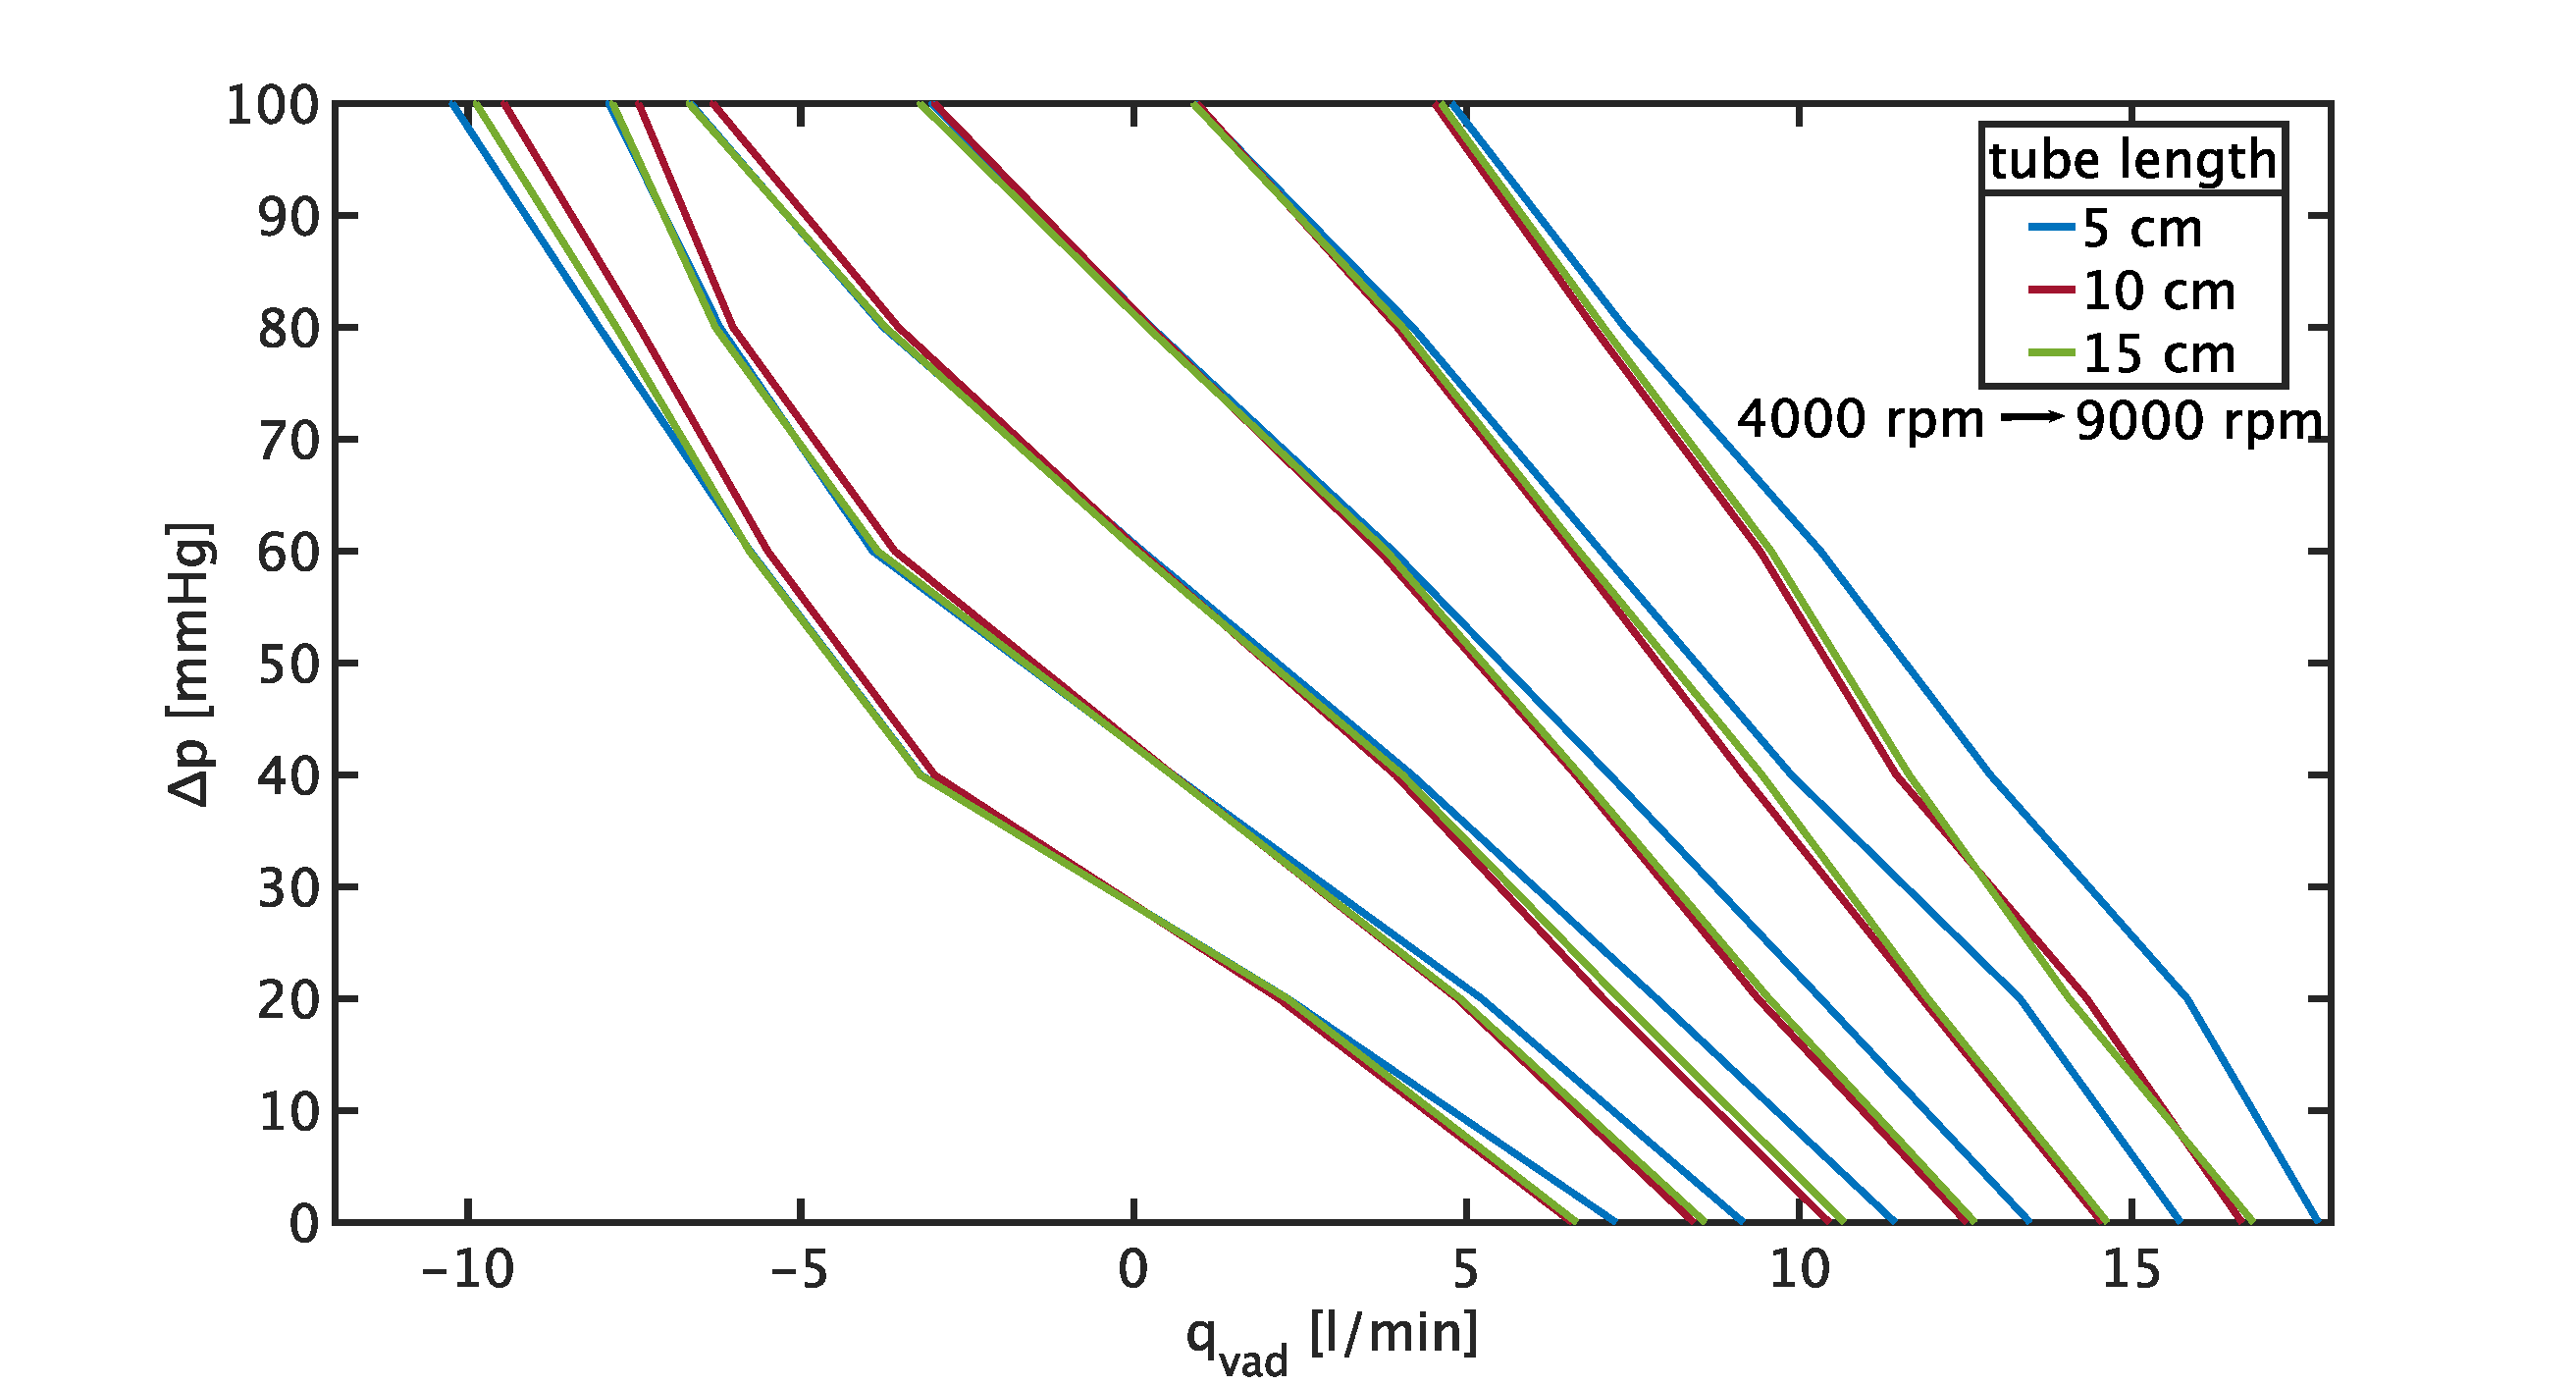
\includegraphics[width=\textwidth]{images/chapt_4/100w_tube_length_new.pdf}
  \caption[Static map for different tube length in 100 \% water]{Static map for varying tube length in 100 \% water}
  \label{fig:anh_1}
\end{figure}

\begin{figure}[ht!]
  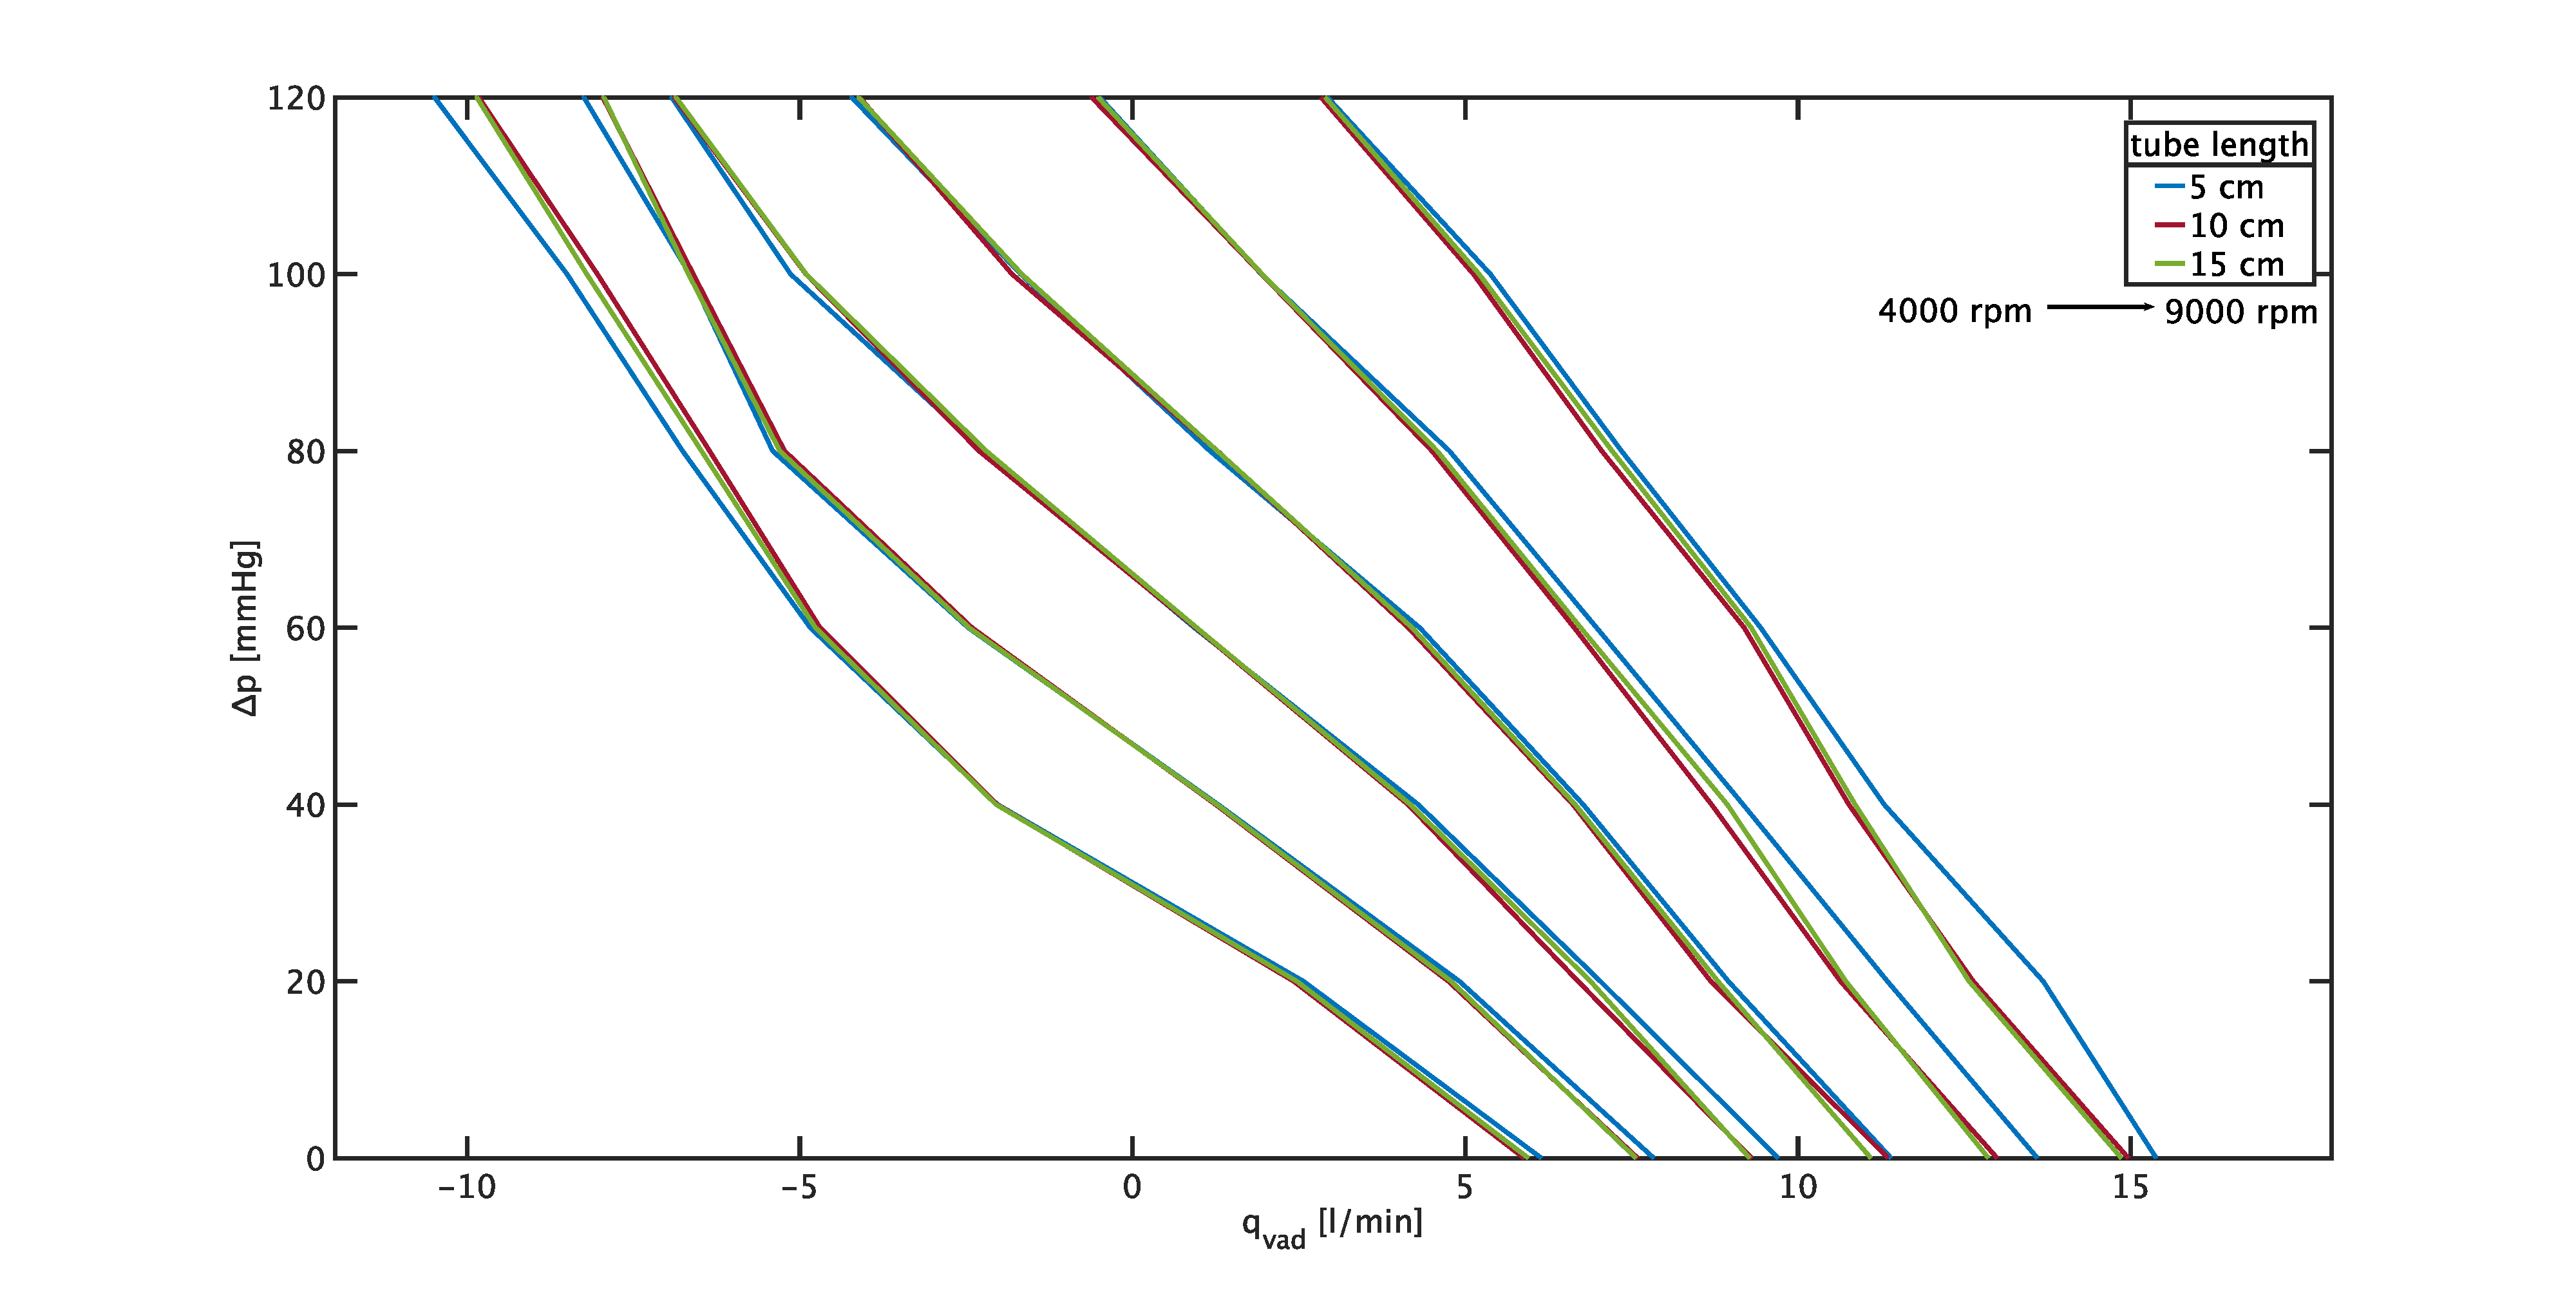
\includegraphics[width=\textwidth]{images/chapt_4/80w20g_tube_length_new.pdf}
  \caption[Static map for different tube length in 80 \% water 20 \% glycerin solution]{Static map for varying tube length in 80 \% water 20 \% glycerin solution}
 \label{fig:anh_2}
\end{figure}

\begin{figure}[ht!]
  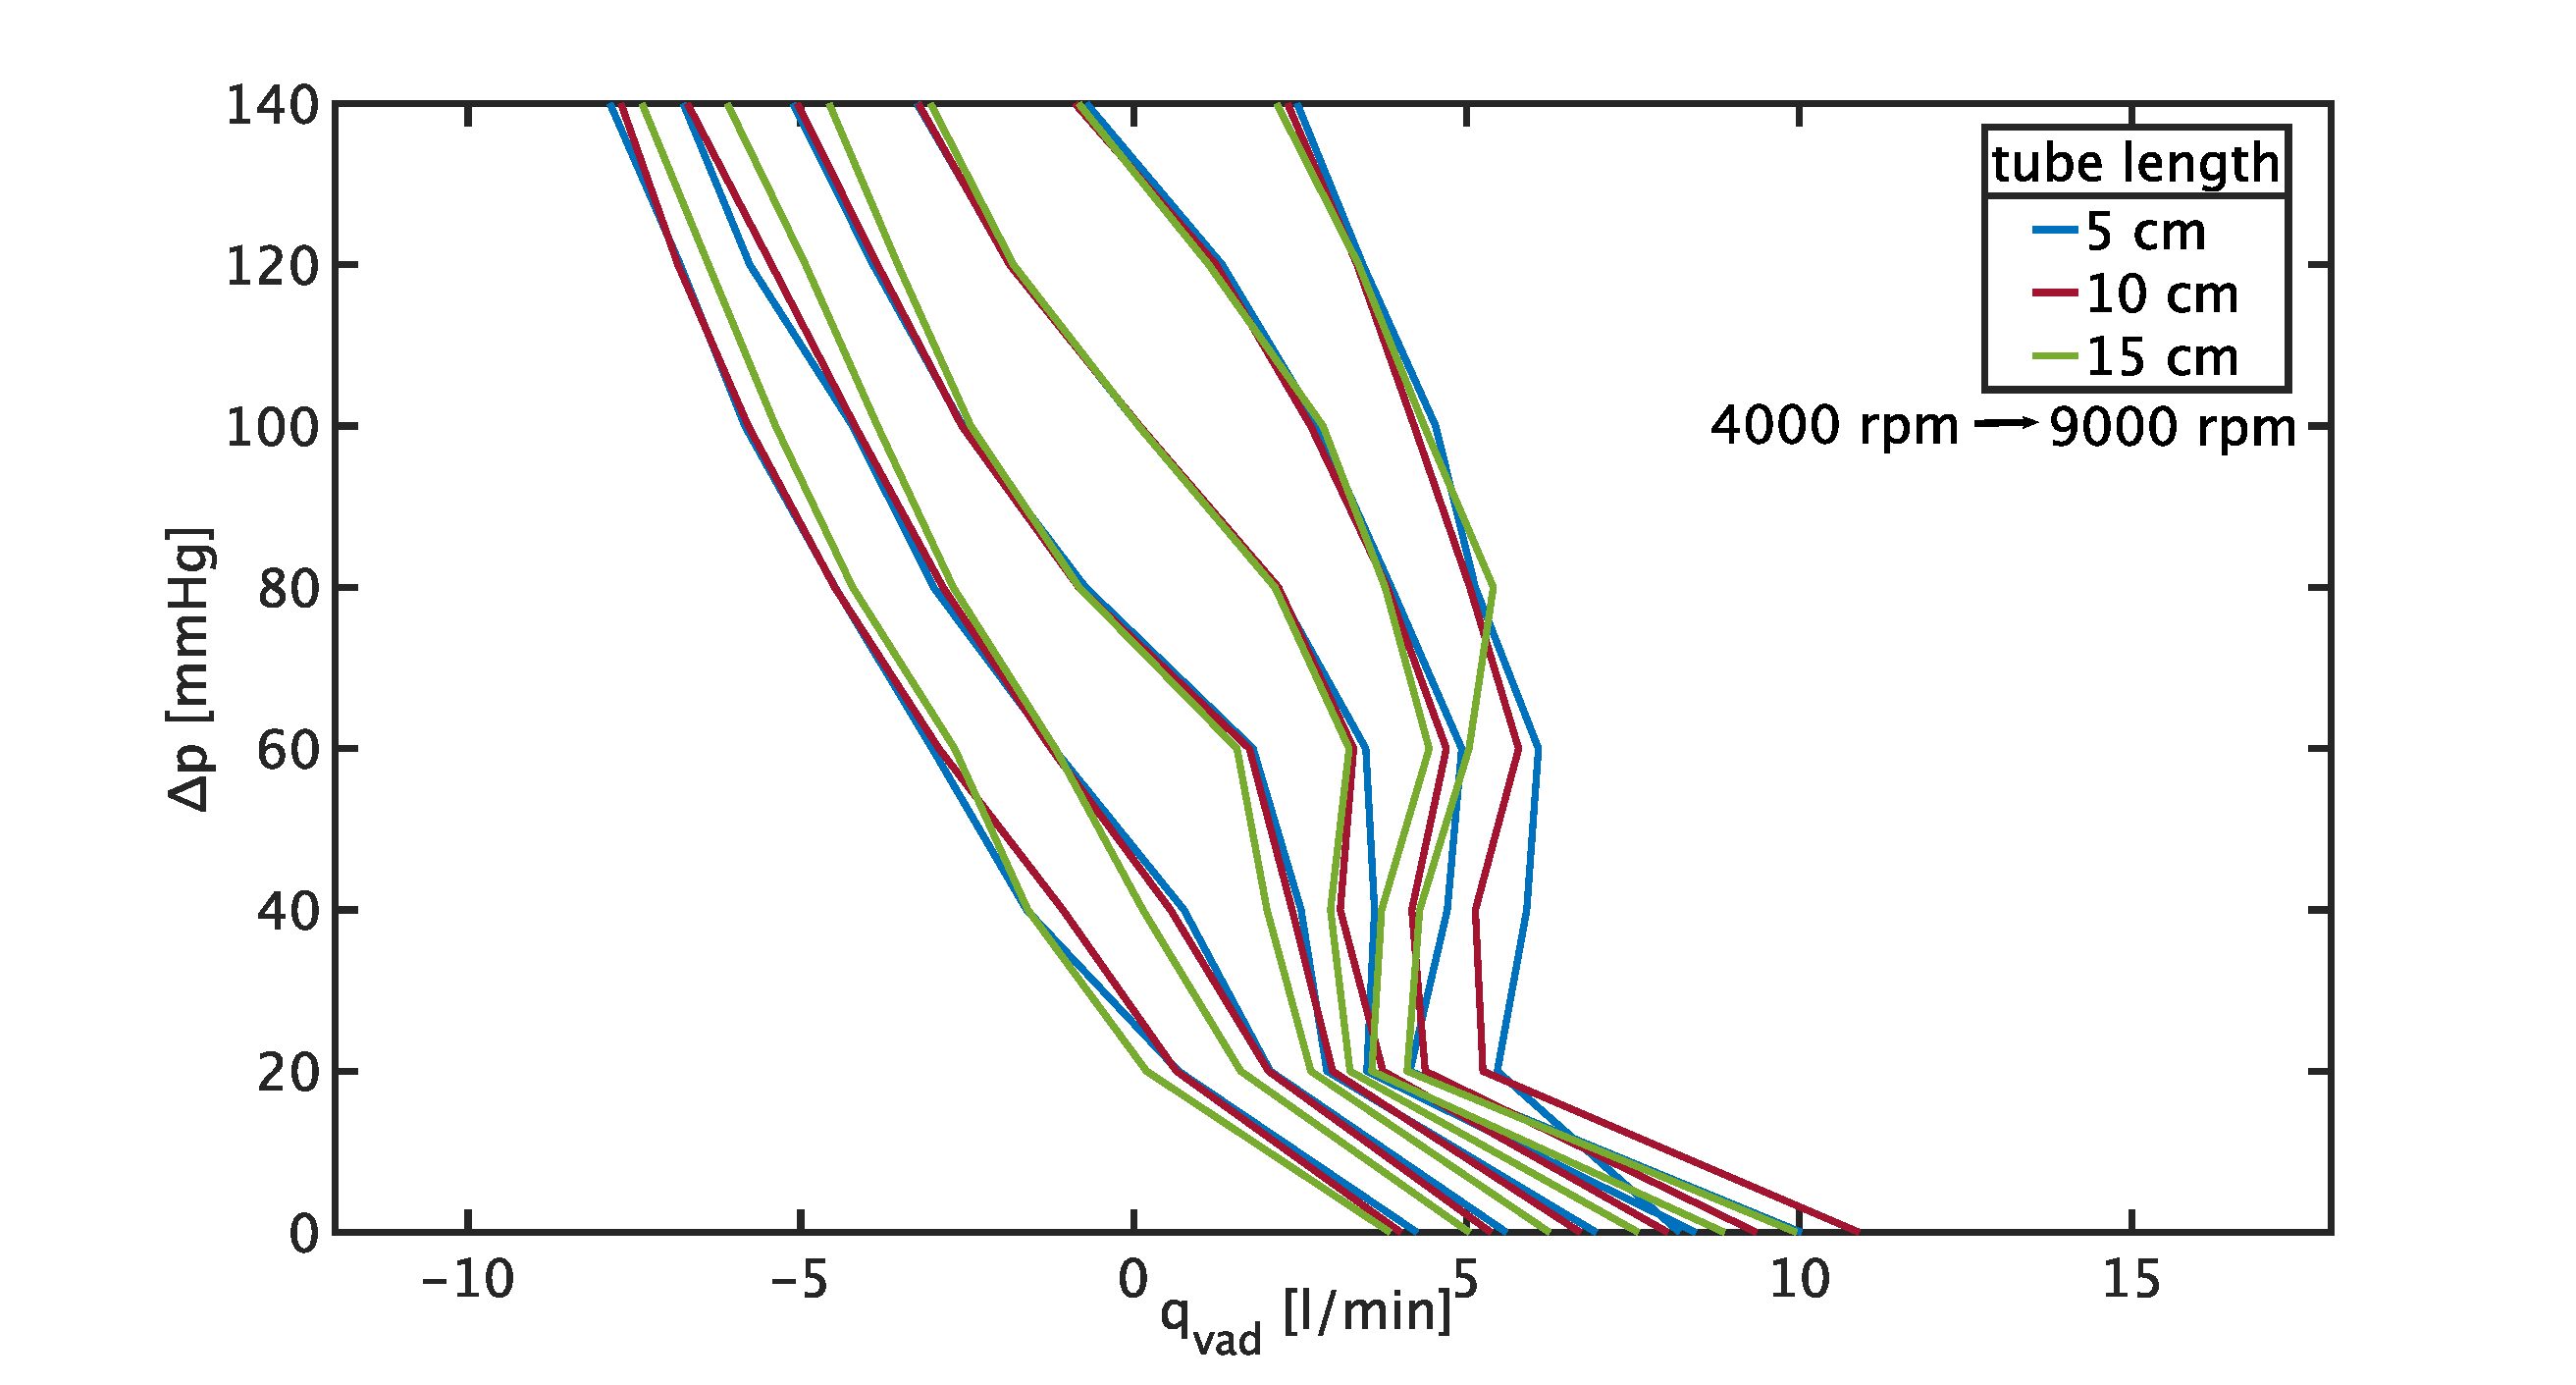
\includegraphics[width=\textwidth]{images/chapt_4/40w60g_tube_length_new.pdf}
  \caption[Static map for different tube length in 40 \% water 60 \% glycerin solution]{Static map for varying tube length in 40 \% water 60 \% glycerin solution}
    \label{fig:anh_3}
\end{figure}

\begin{figure}[ht!]
  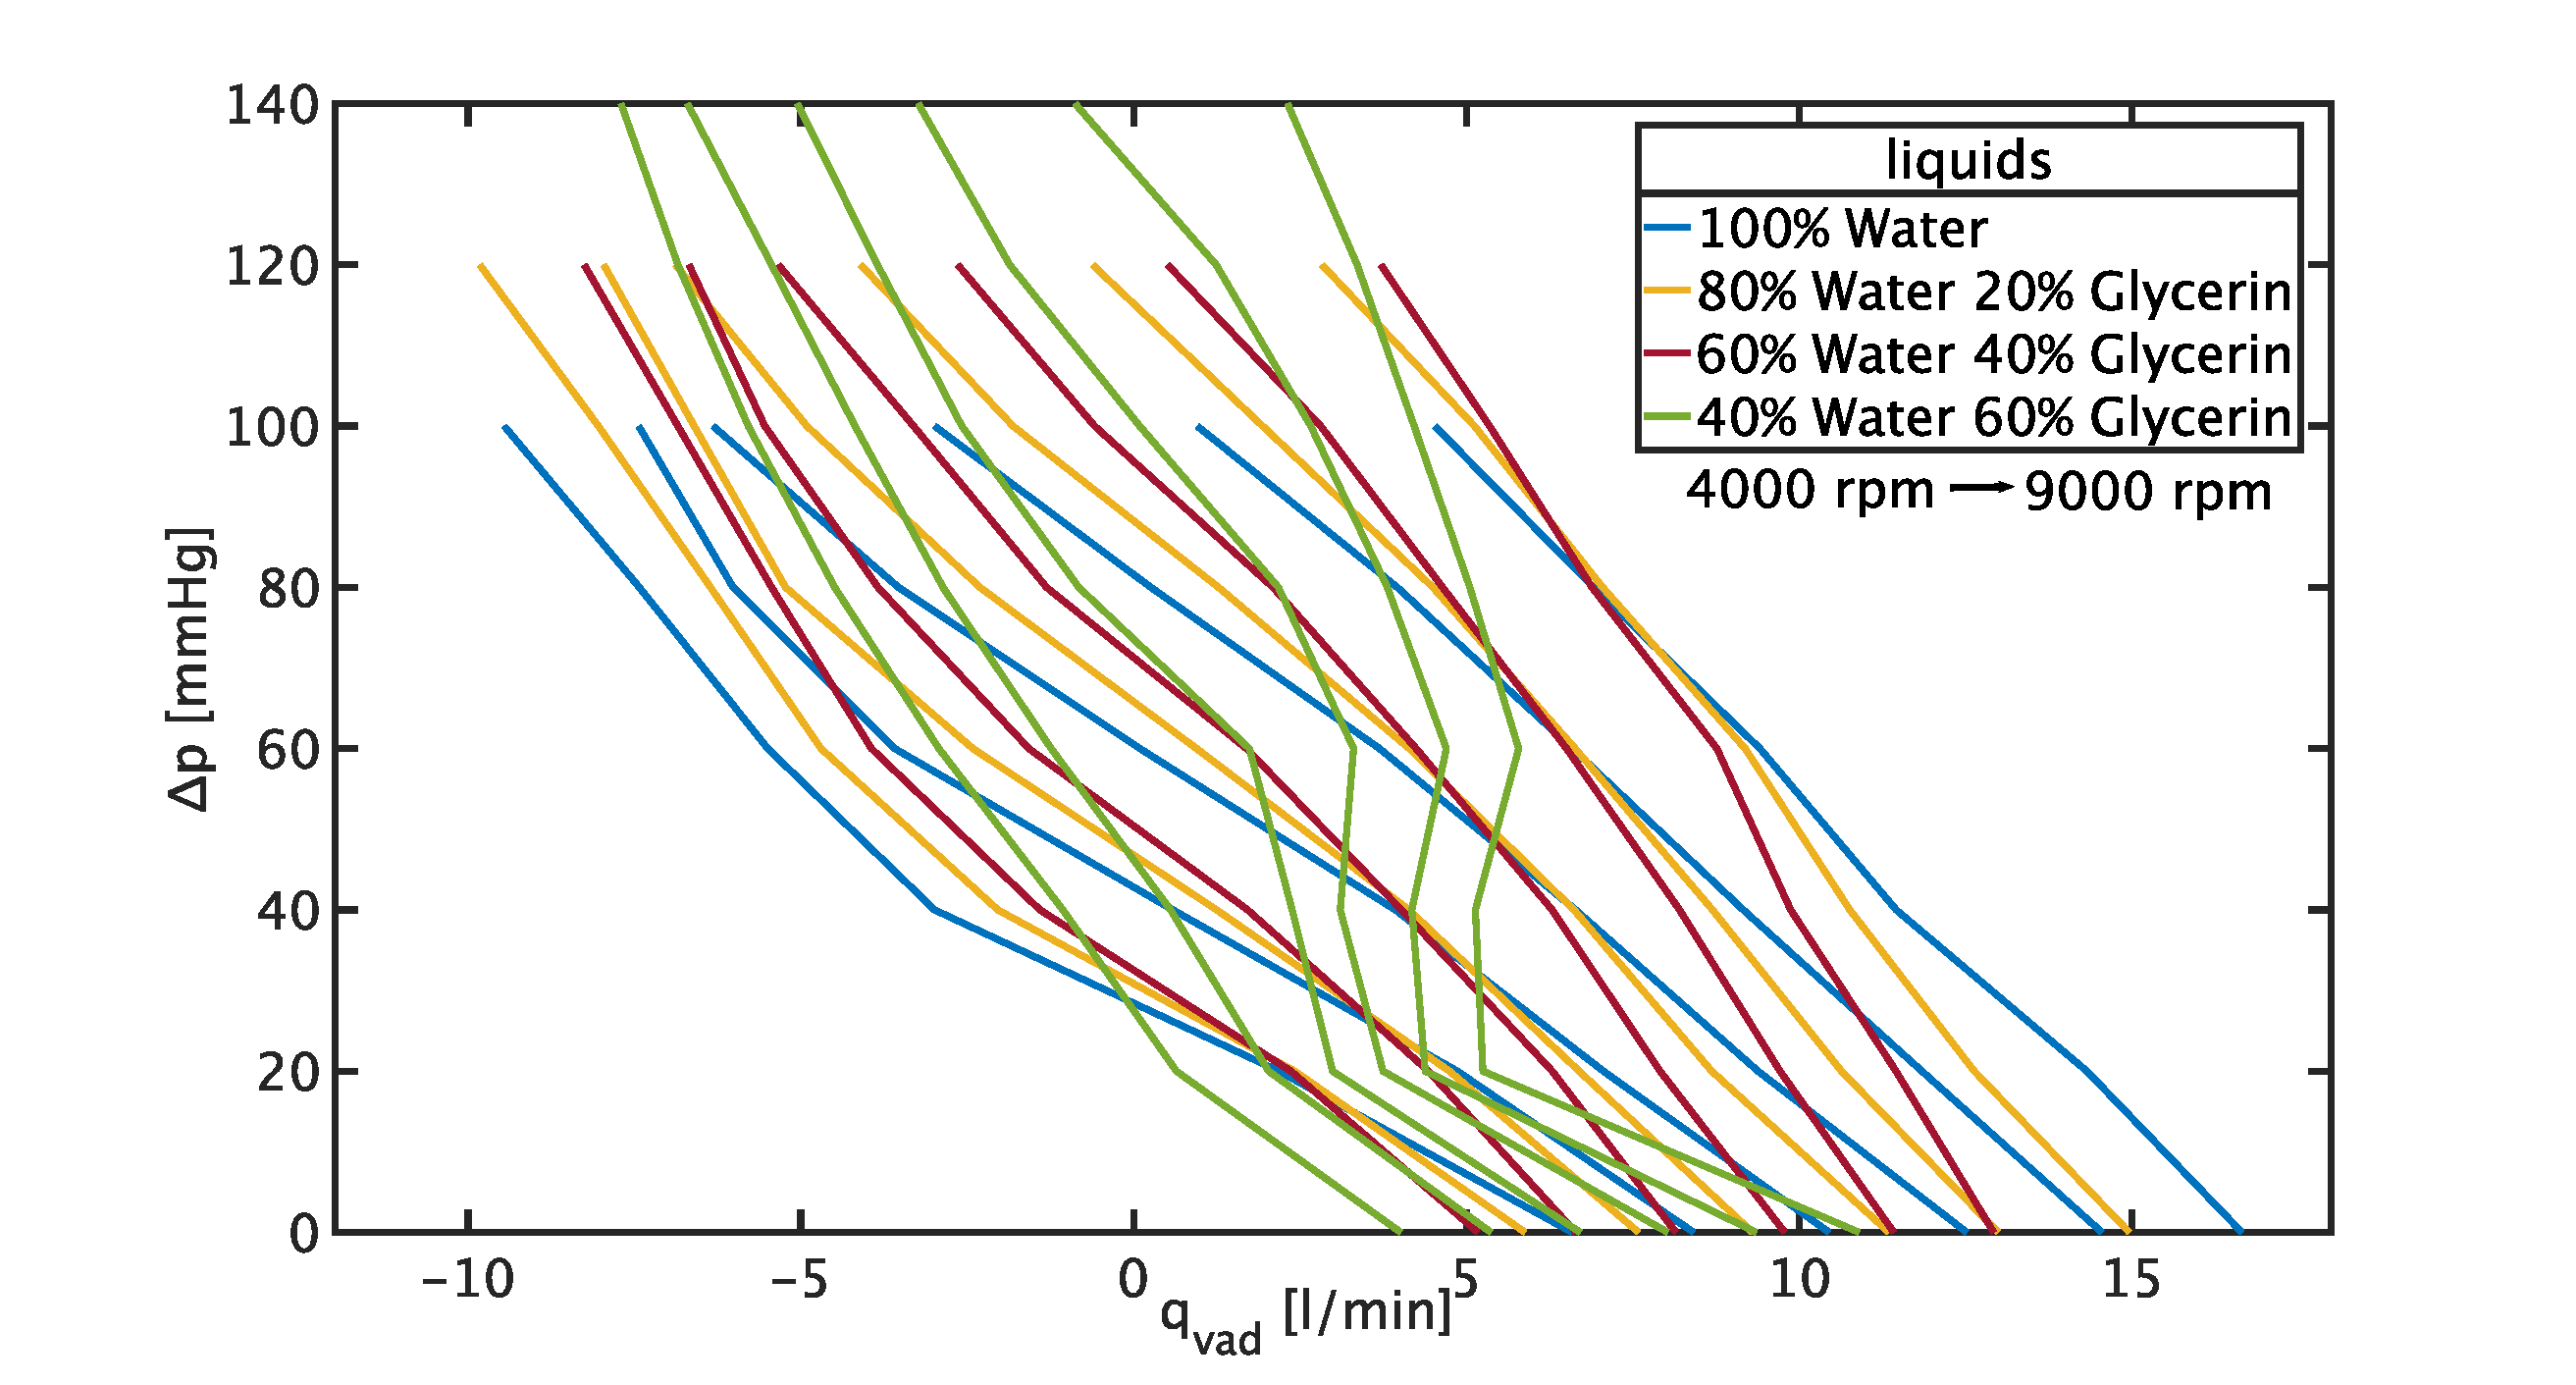
\includegraphics[width=\textwidth]{images/chapt_4/medium_liquid_change_new.pdf}
  \caption[Static map for varying liquid solutions with $10\,cm$ tube length]{Static map for varying liquid solutions with $10\,cm$ tube length.}
    \label{fig:anh_4}
\end{figure}

\begin{figure}[ht!]
  \includegraphics[width=\textwidth]{images/chapt_4/short_liquid_change_new.pdf}
  \caption[Static map for varying liquid solutions with $5\,cm$ tube length]{Static map for varying liquid solutions with $5\,cm$ tube length.}
    \label{fig:anh_5}
\end{figure}

 %\section{Flow Control}
% \subsection{PI Controllers}\label{A2_1}
\begin{figure}[ht!]
  \centering
  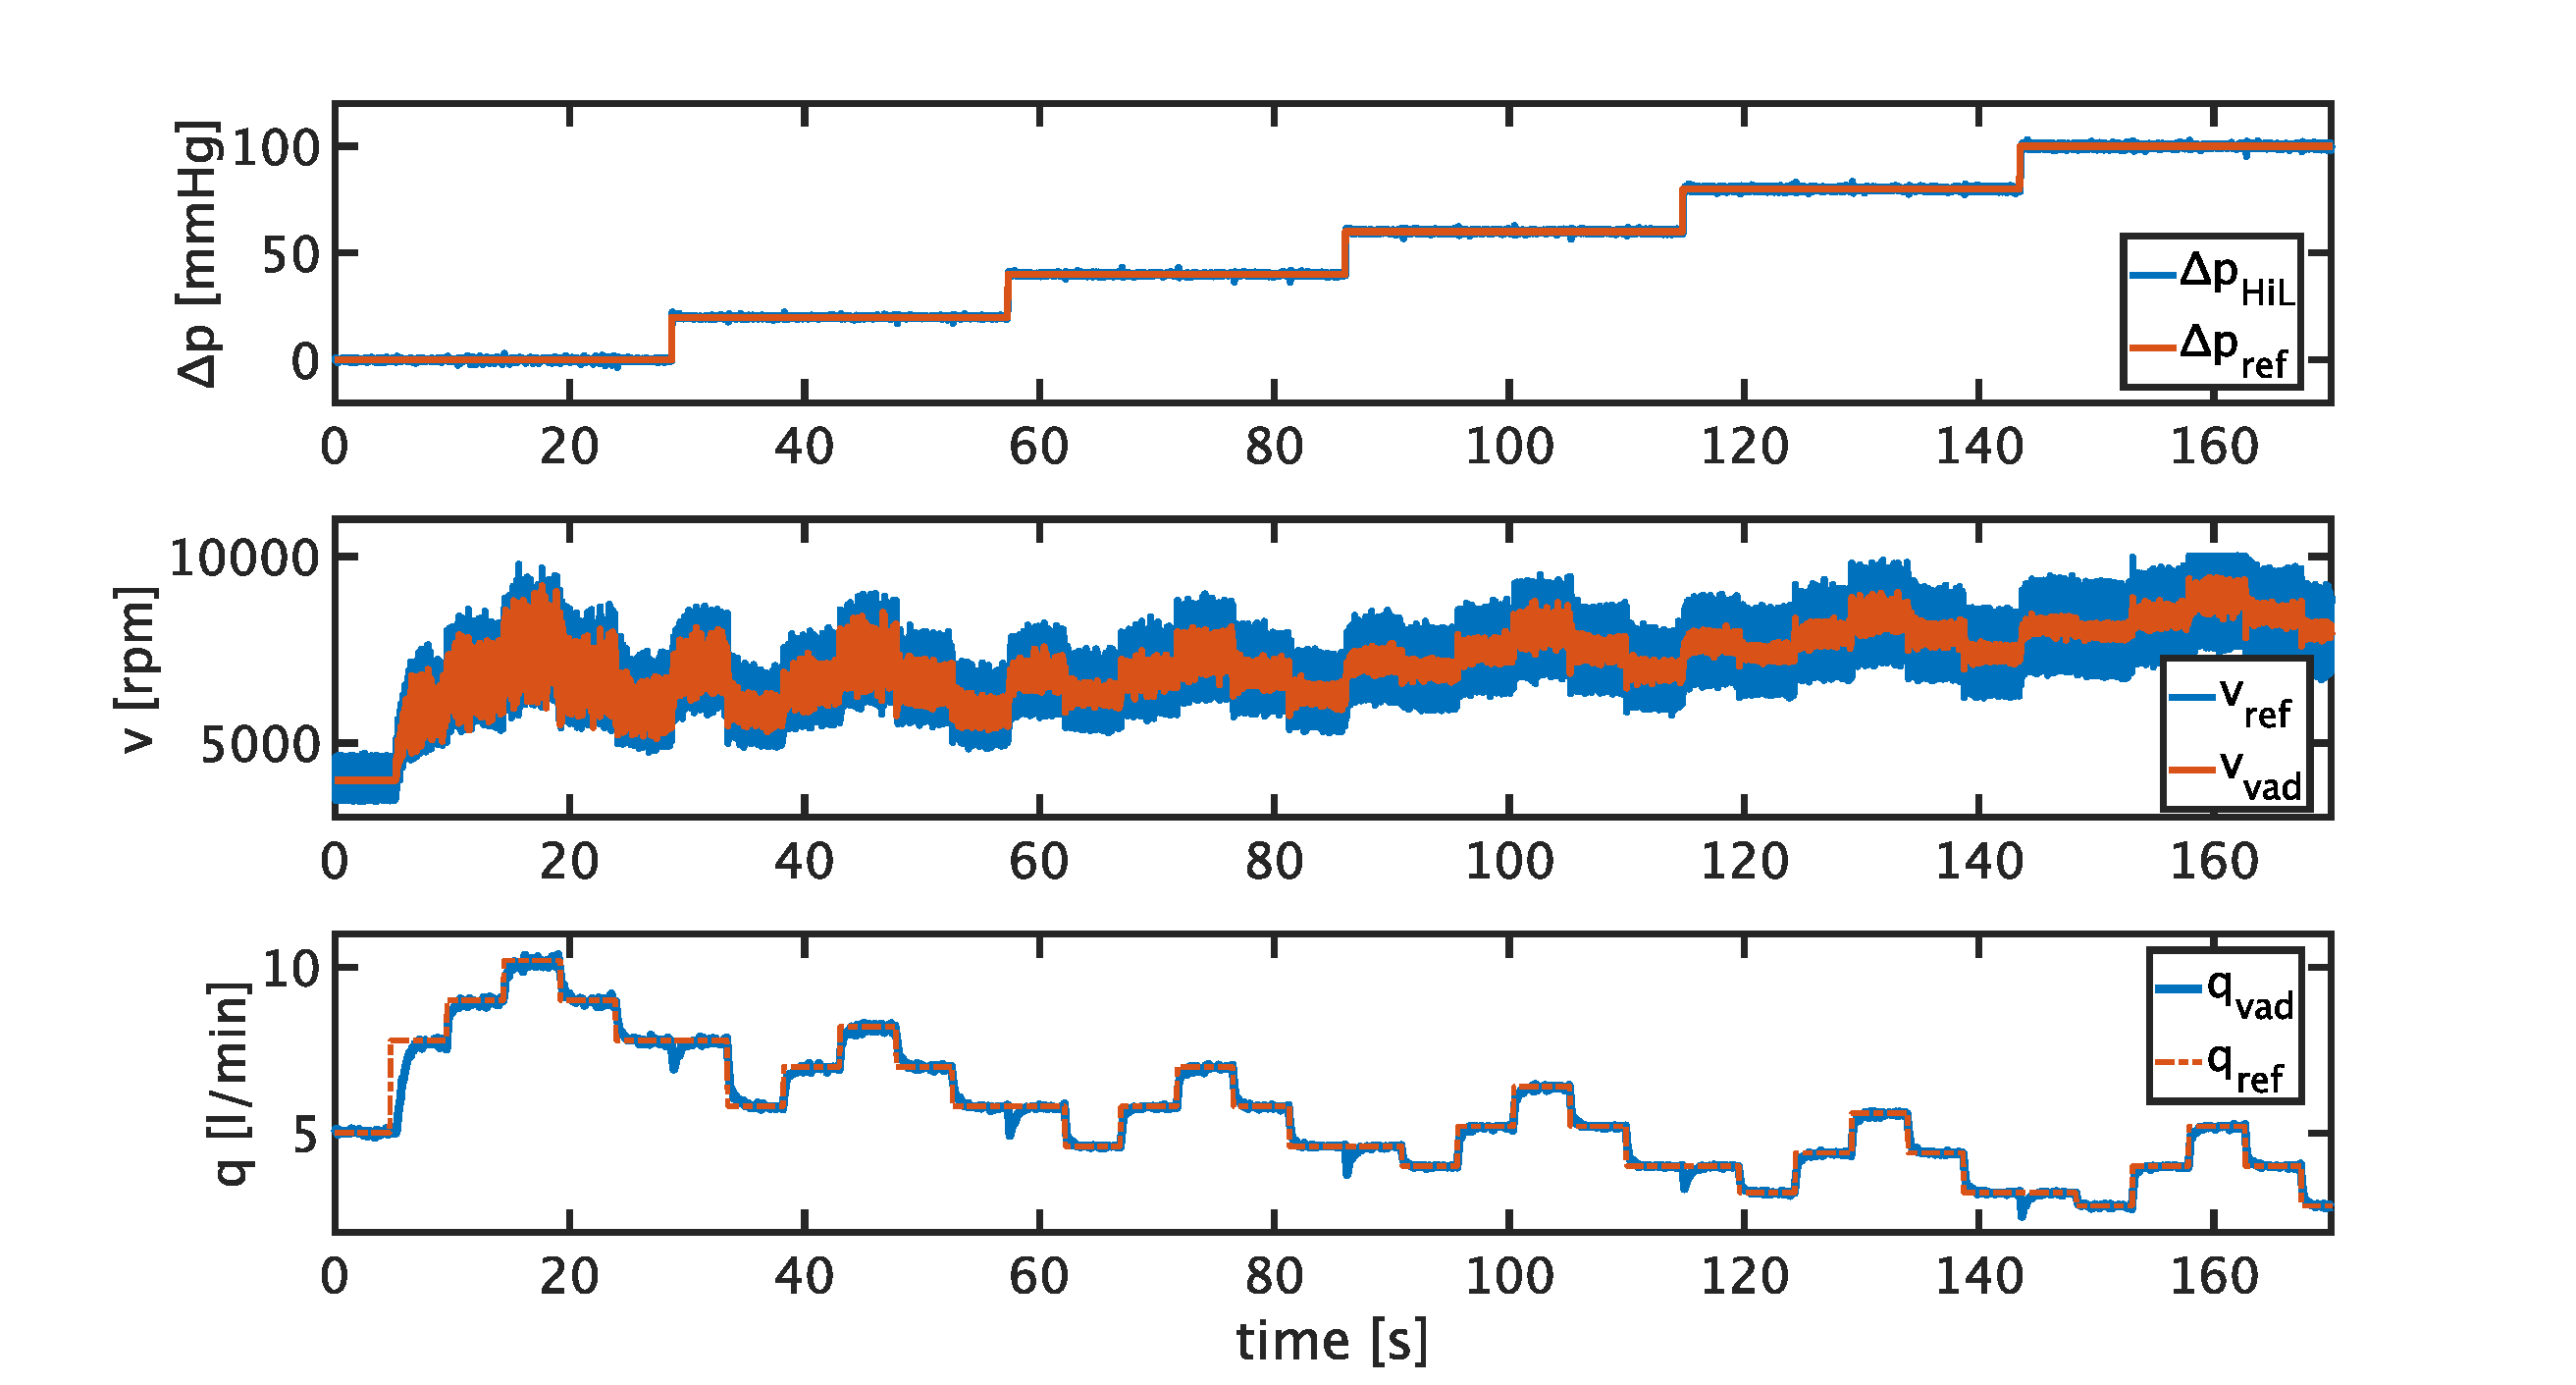
\includegraphics[width=\textwidth]{images/chapt_5/pi_contr_chr.pdf}
  \caption[Test measurement for PI controller tuned according to Chien Hrones Reswick]{Test measurement for PI controller tuned according to Chien Hrones Reswick.}
  \label{fig:anh_6}
\end{figure}

\begin{figure}[ht!]
  \centering
  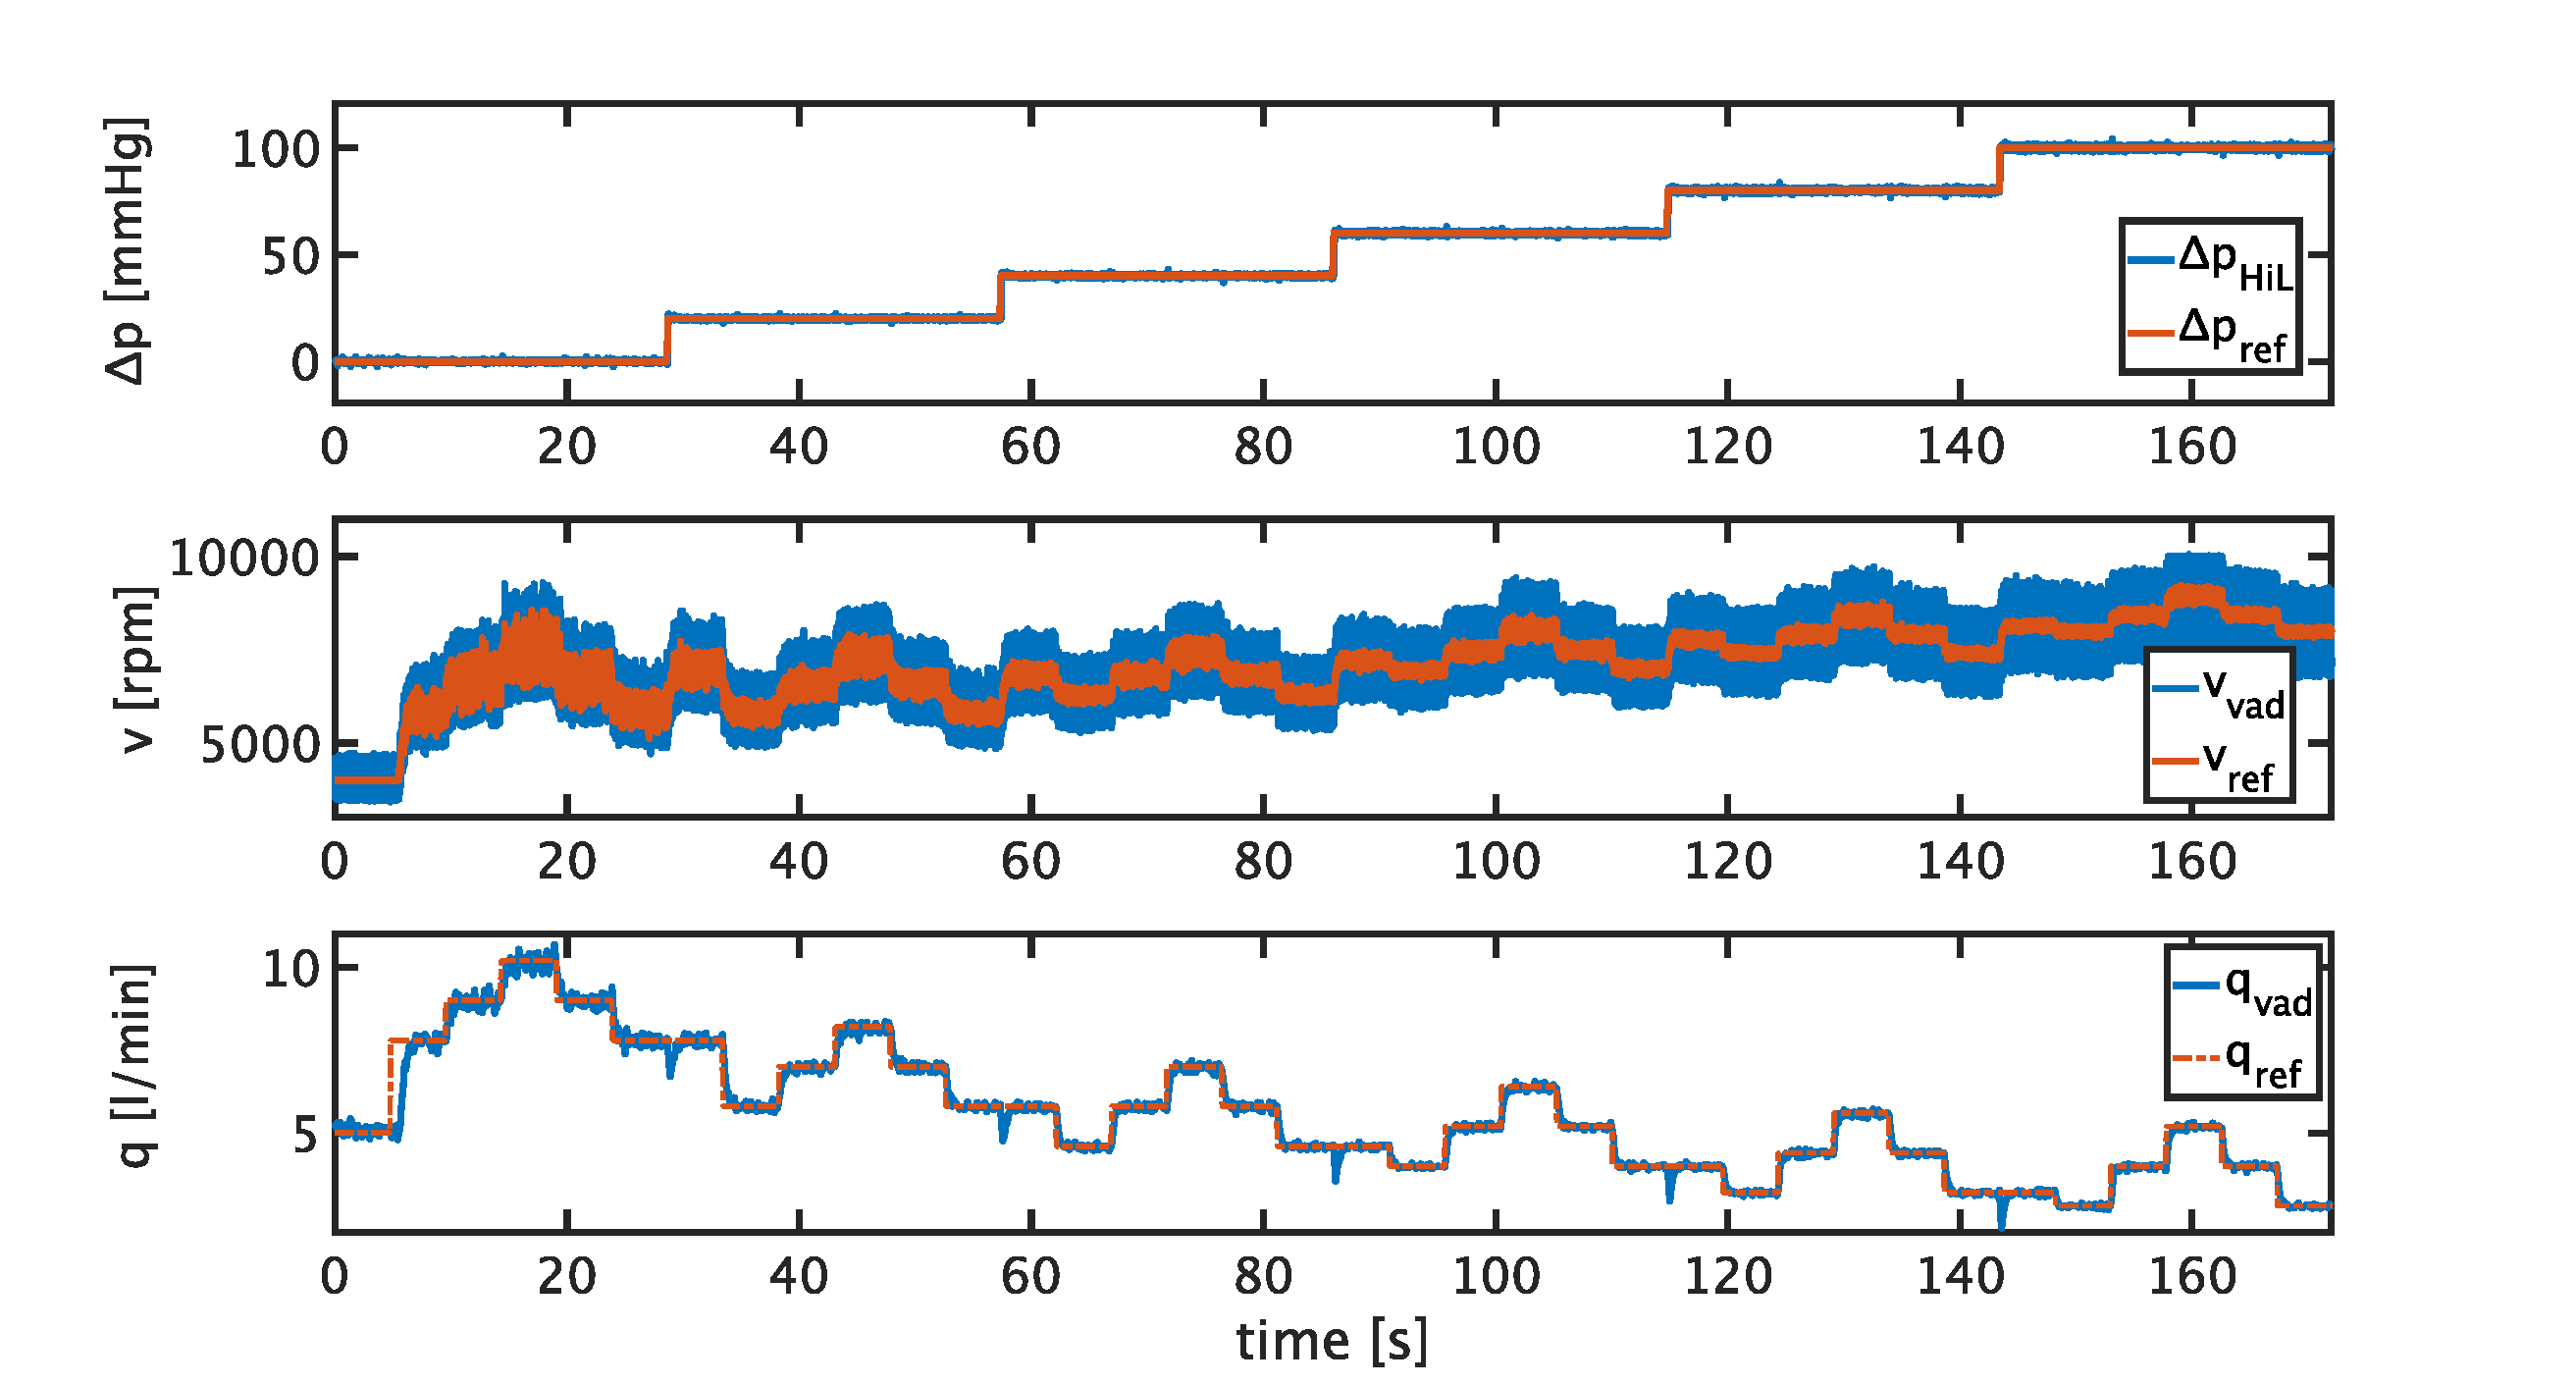
\includegraphics[width=\textwidth]{images/chapt_5/pi_contr_zn.pdf}
  \caption[Test measurement for PI controller tuned according to Ziegler Nichols]{Test measurement for PI controller tuned according to Ziegler Nichols.}
  \label{fig:anh_7}
\end{figure}

\begin{figure}[ht!]
  \centering
  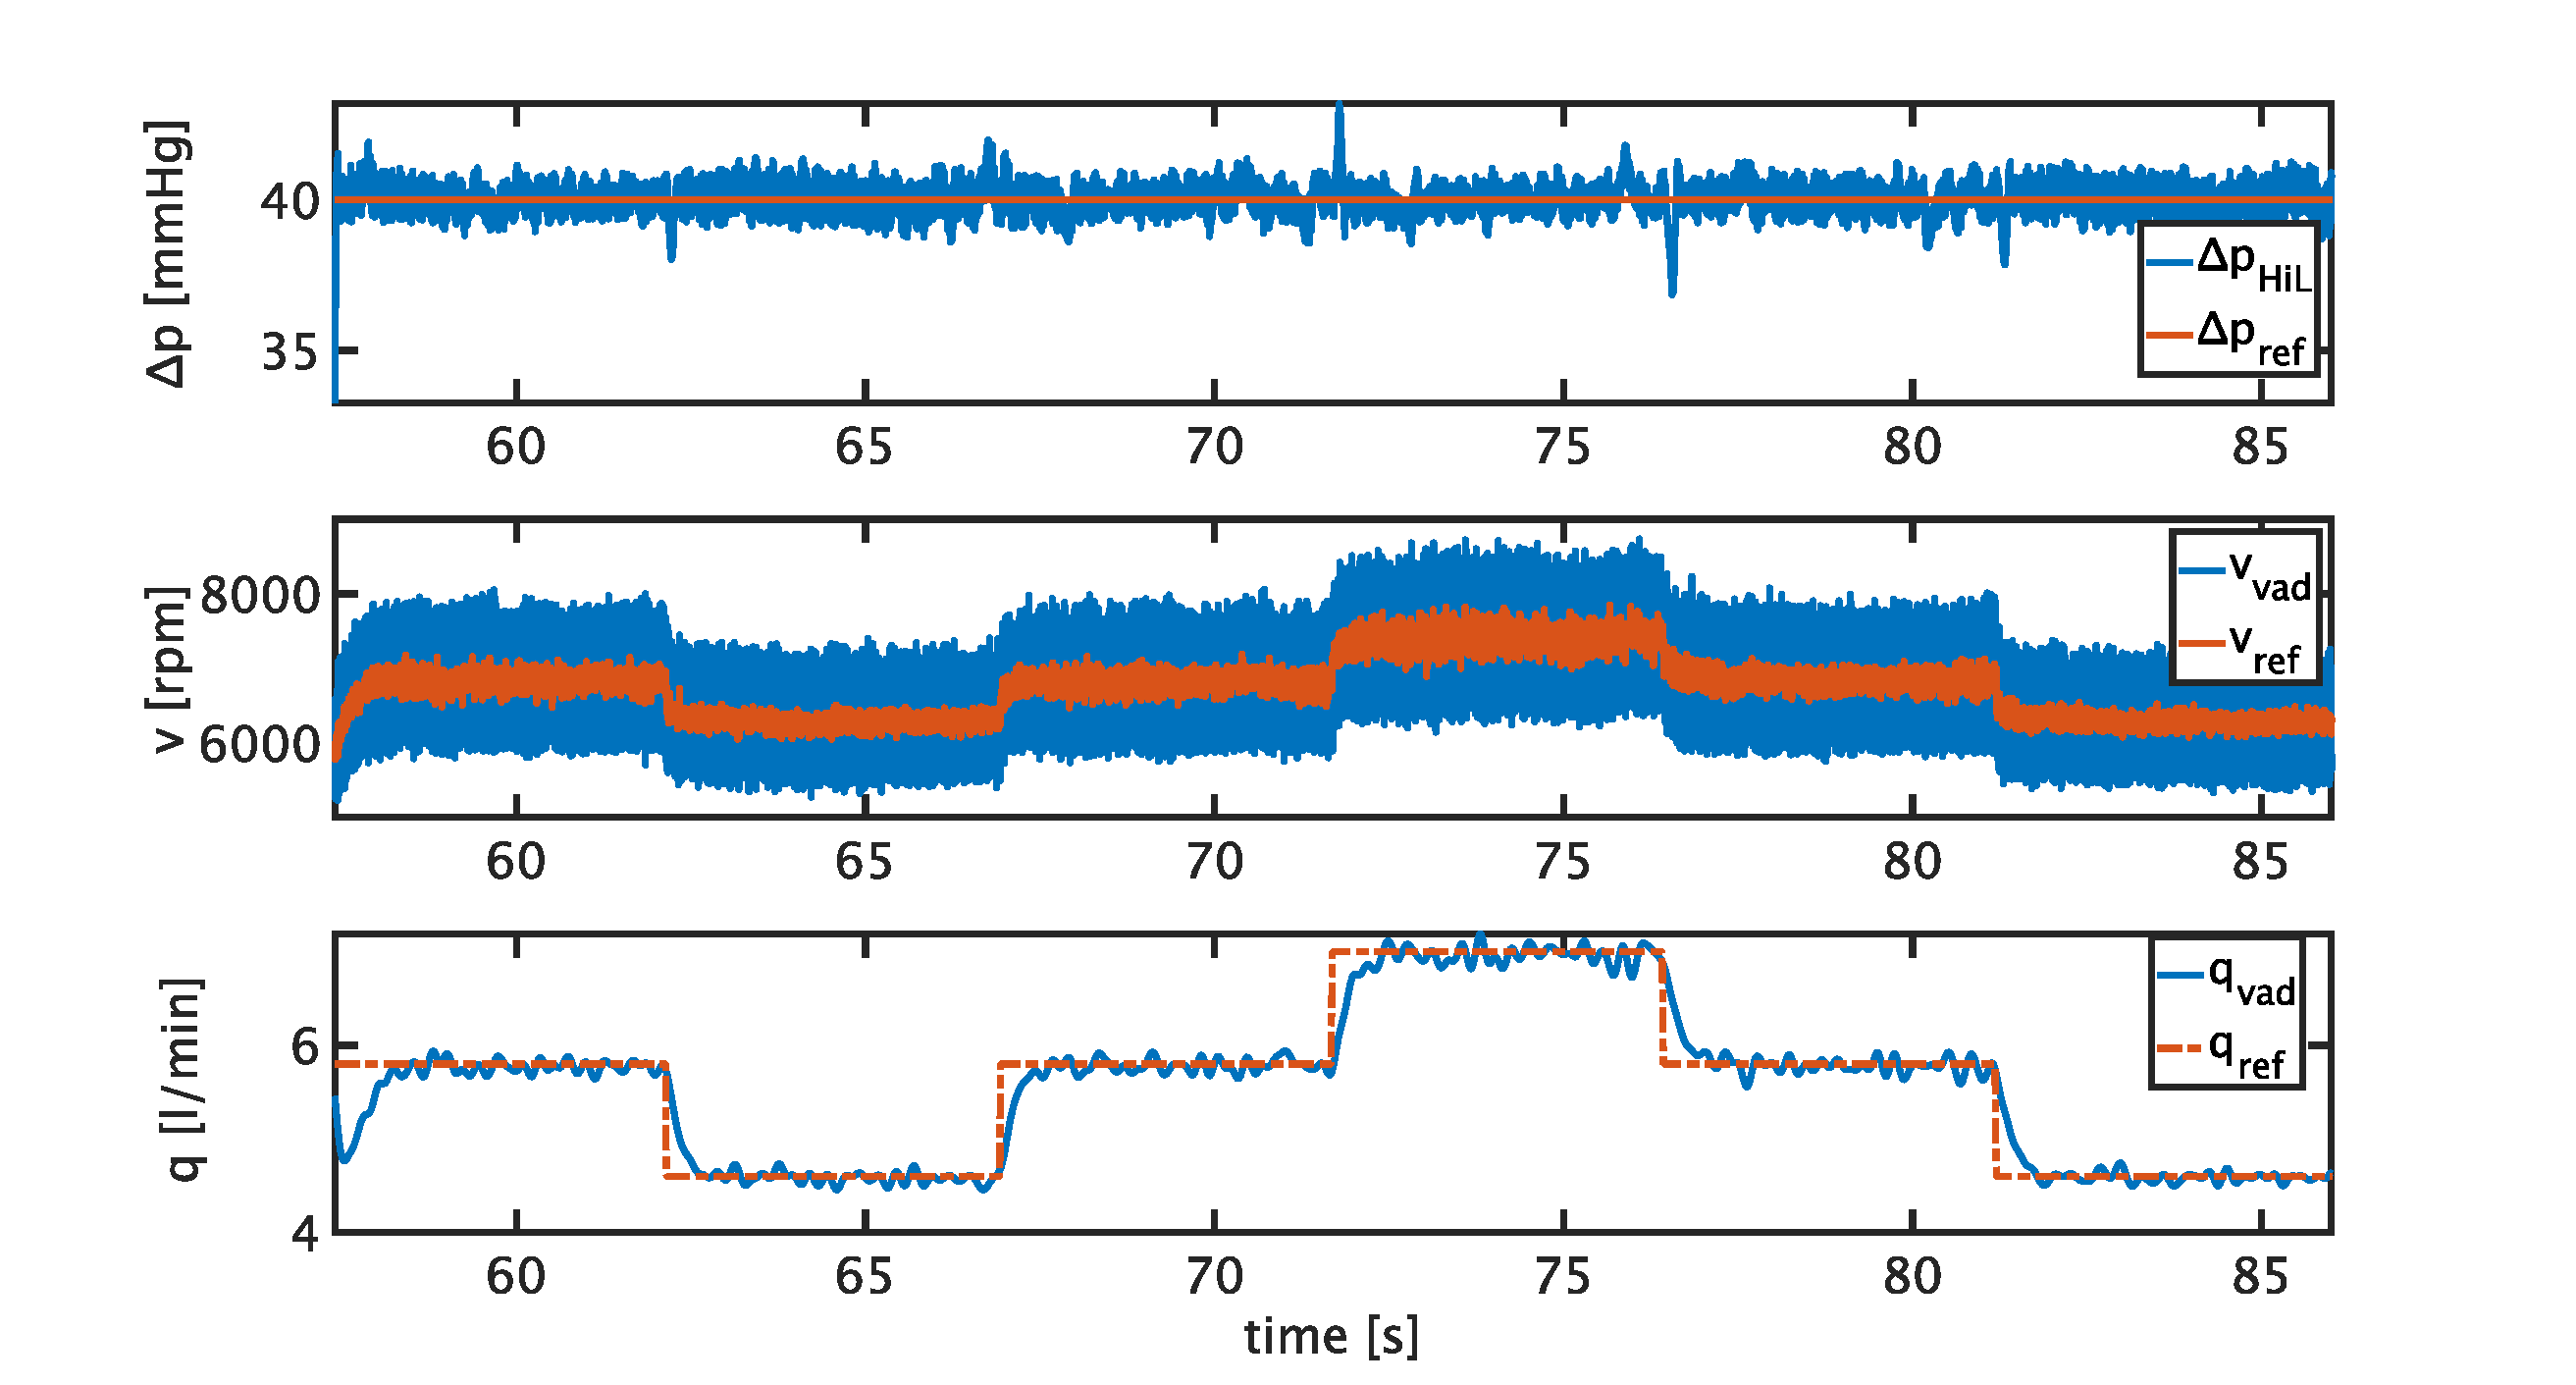
\includegraphics[width=\textwidth]{images/chapt_5/pi_contr_zn_40.pdf}
  \caption[Test measurement for PI controller tuned according to Ziegler Nichols at $\Delta{p}=40\,mmHg$]{Test measurement for PI controller tuned according to Ziegler Nichols at $\Delta{p}=40\,mmHg$.}
  \label{fig:anh_8}
\end{figure}

%\section{ILC with varying disturbance}

\begin{figure}[ht!]
  \centering
  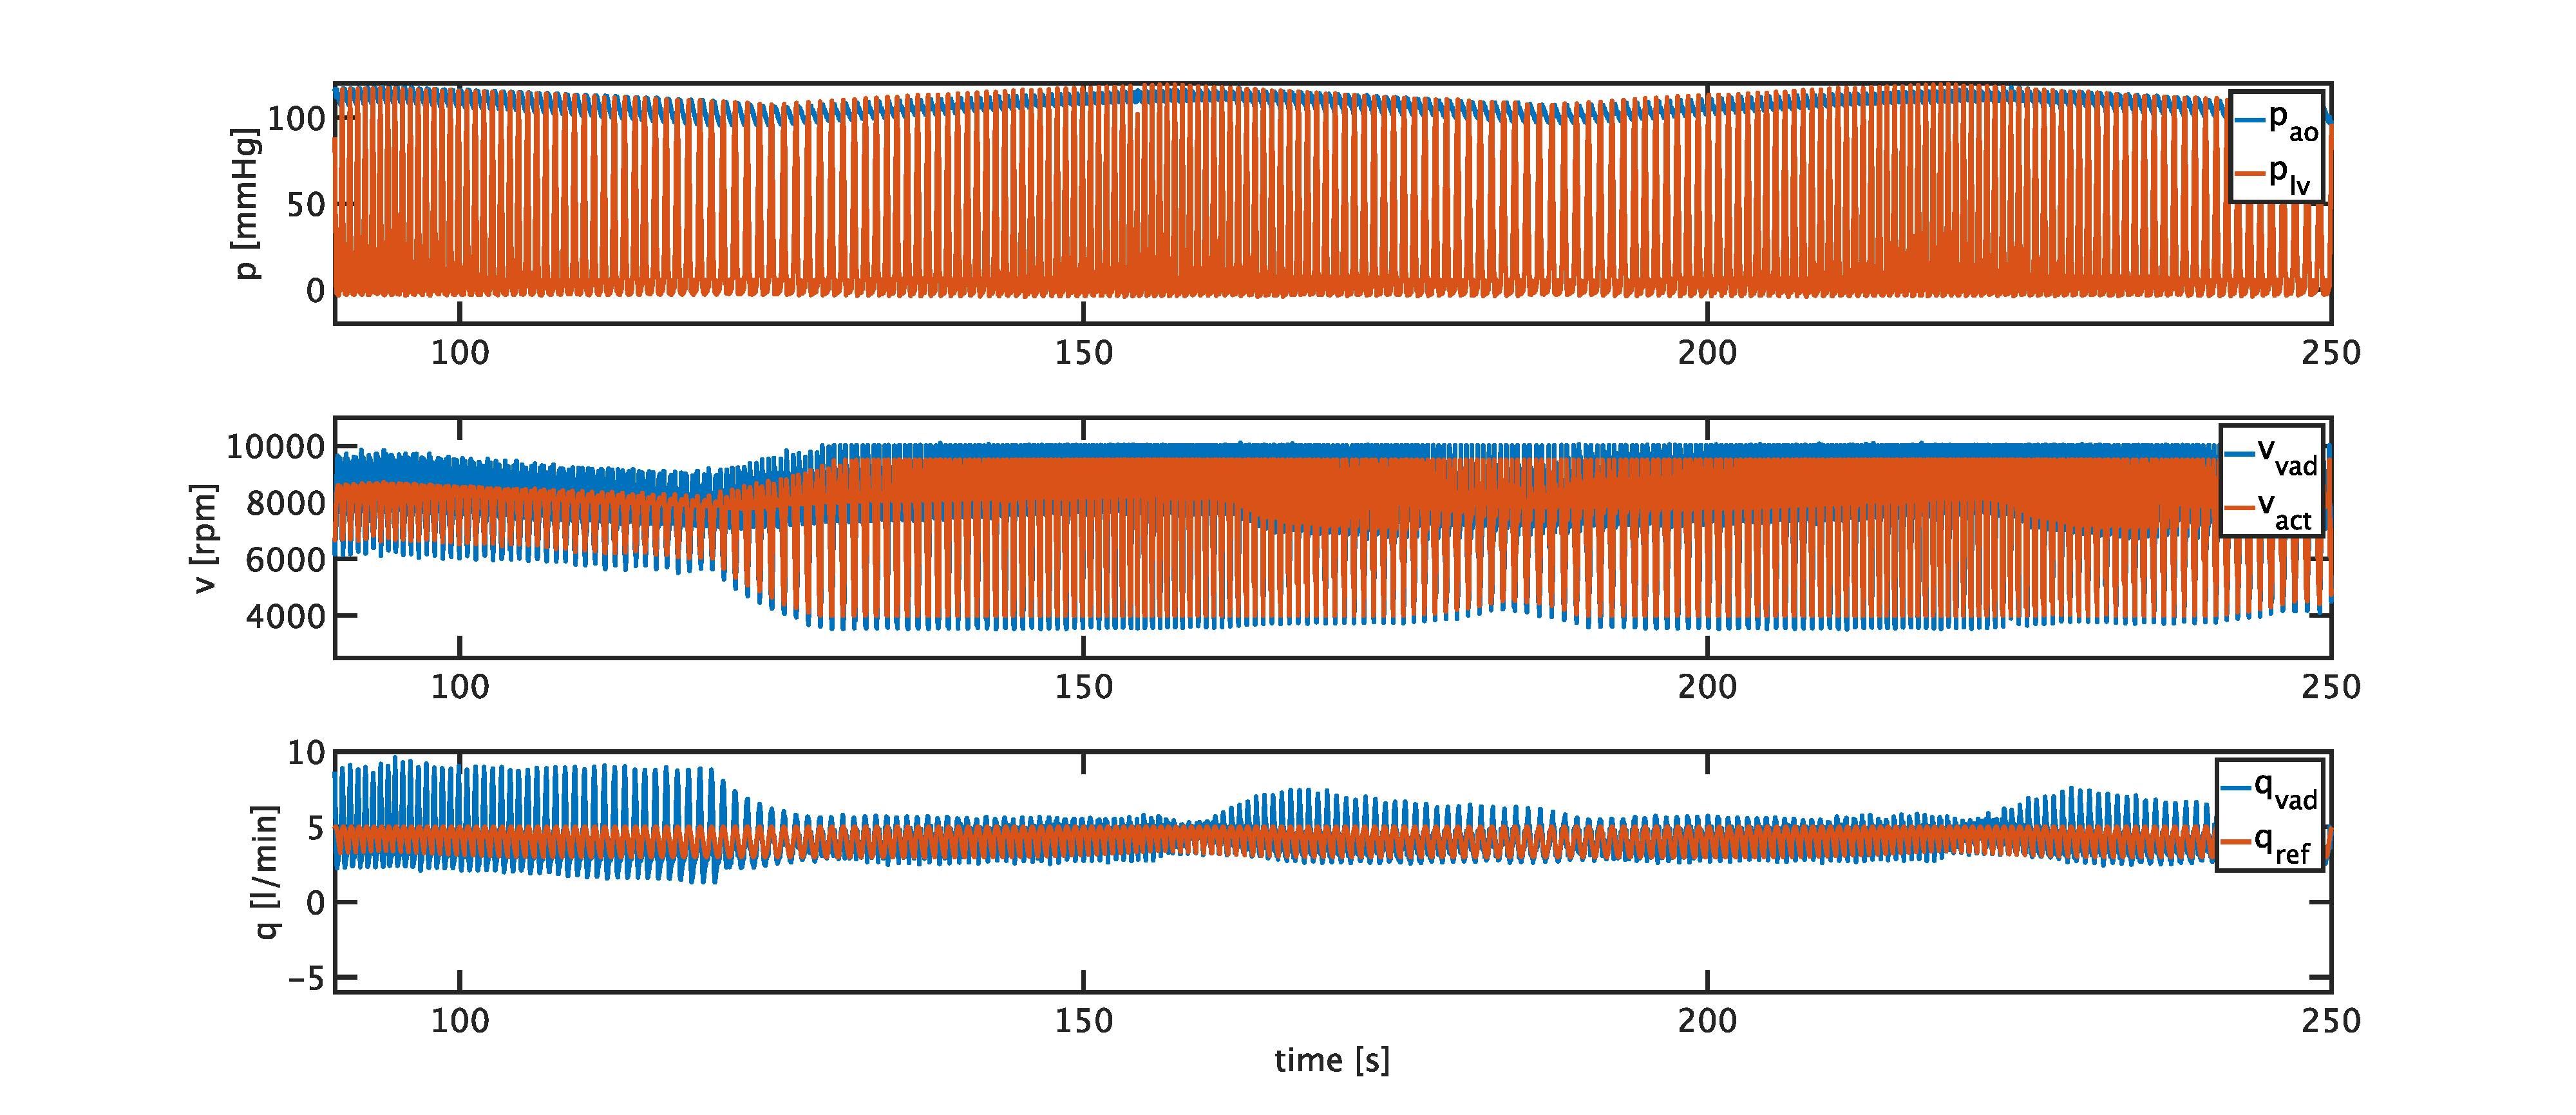
\includegraphics[width=0.95\textwidth]{images/chapt_5/ILC/ilc_var_dist_unfix_sine.pdf}
  \caption[Segment of measurement for ILC with varying disturbance with $cf_{\mathrm{Lv}}=1$ for sinusoidal reference flow without data resampling]{Segment of measurement for ILC with varying disturbance with $cf_{\mathrm{Lv}}=1$ for sinusoidal reference flow without data resampling. Top:  pressure values of the MCL. Middle: actuating variable and measured rotational speed of the VAD. Bottom: targeted flow trajectory and measured flow through the VAD}
 % \label{fig:ilc_var_dist_unfix_sine}
 \label{fig:anh_9}
\end{figure}

\begin{figure}[ht!]
  \centering
  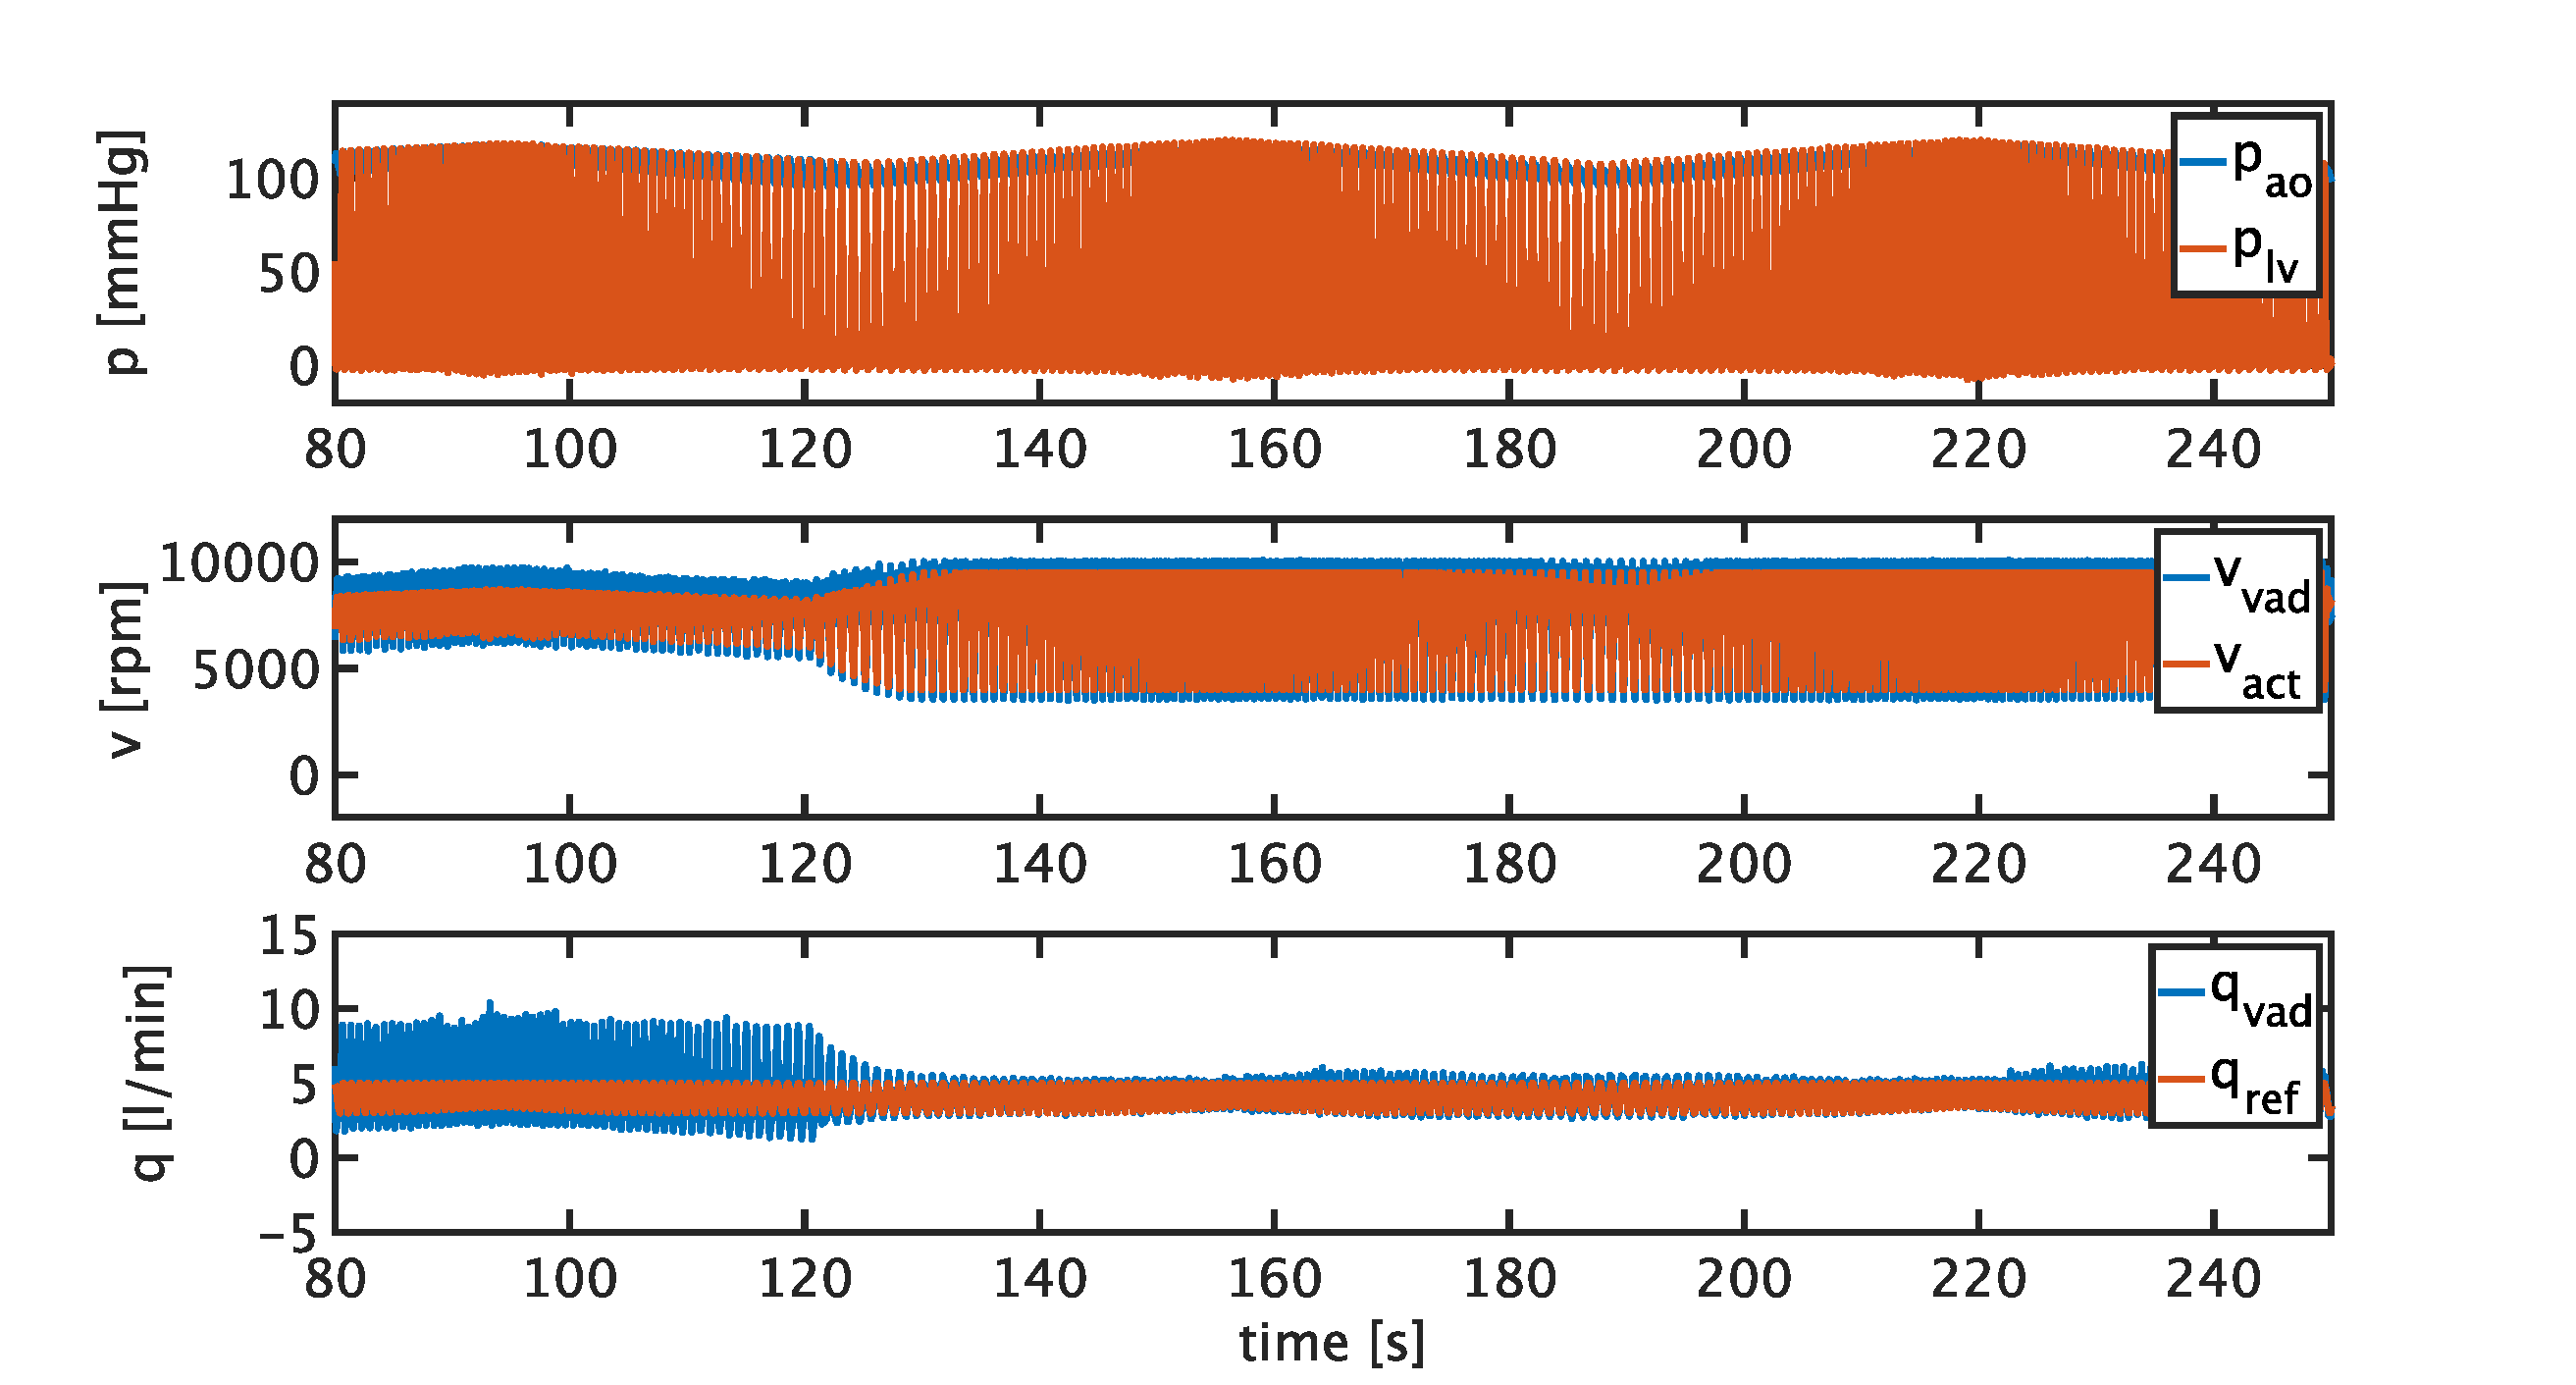
\includegraphics[width=0.95\textwidth]{images/chapt_5/ILC/ilc_var_dist_fix_sine.pdf}
  \caption[Segment of measurement for ILC with varying disturbance with $cf_{\mathrm{Lv}}=1$ for sinusoidal reference flow with data resampling]{Segment of measurement for ILC with varying disturbance with $cf_{\mathrm{Lv}}=1$ for sinusoidal reference flow with data resampling. Top:  pressure values of the MCL. Middle: actuating variable and measured rotational speed of the VAD. Bottom: targeted flow trajectory and measured flow through the VAD}
  %\label{fig:ilc_var_dist_fix_sine}
   \label{fig:anh_10}
\end{figure}

\begin{figure}[ht!]
  \centering
  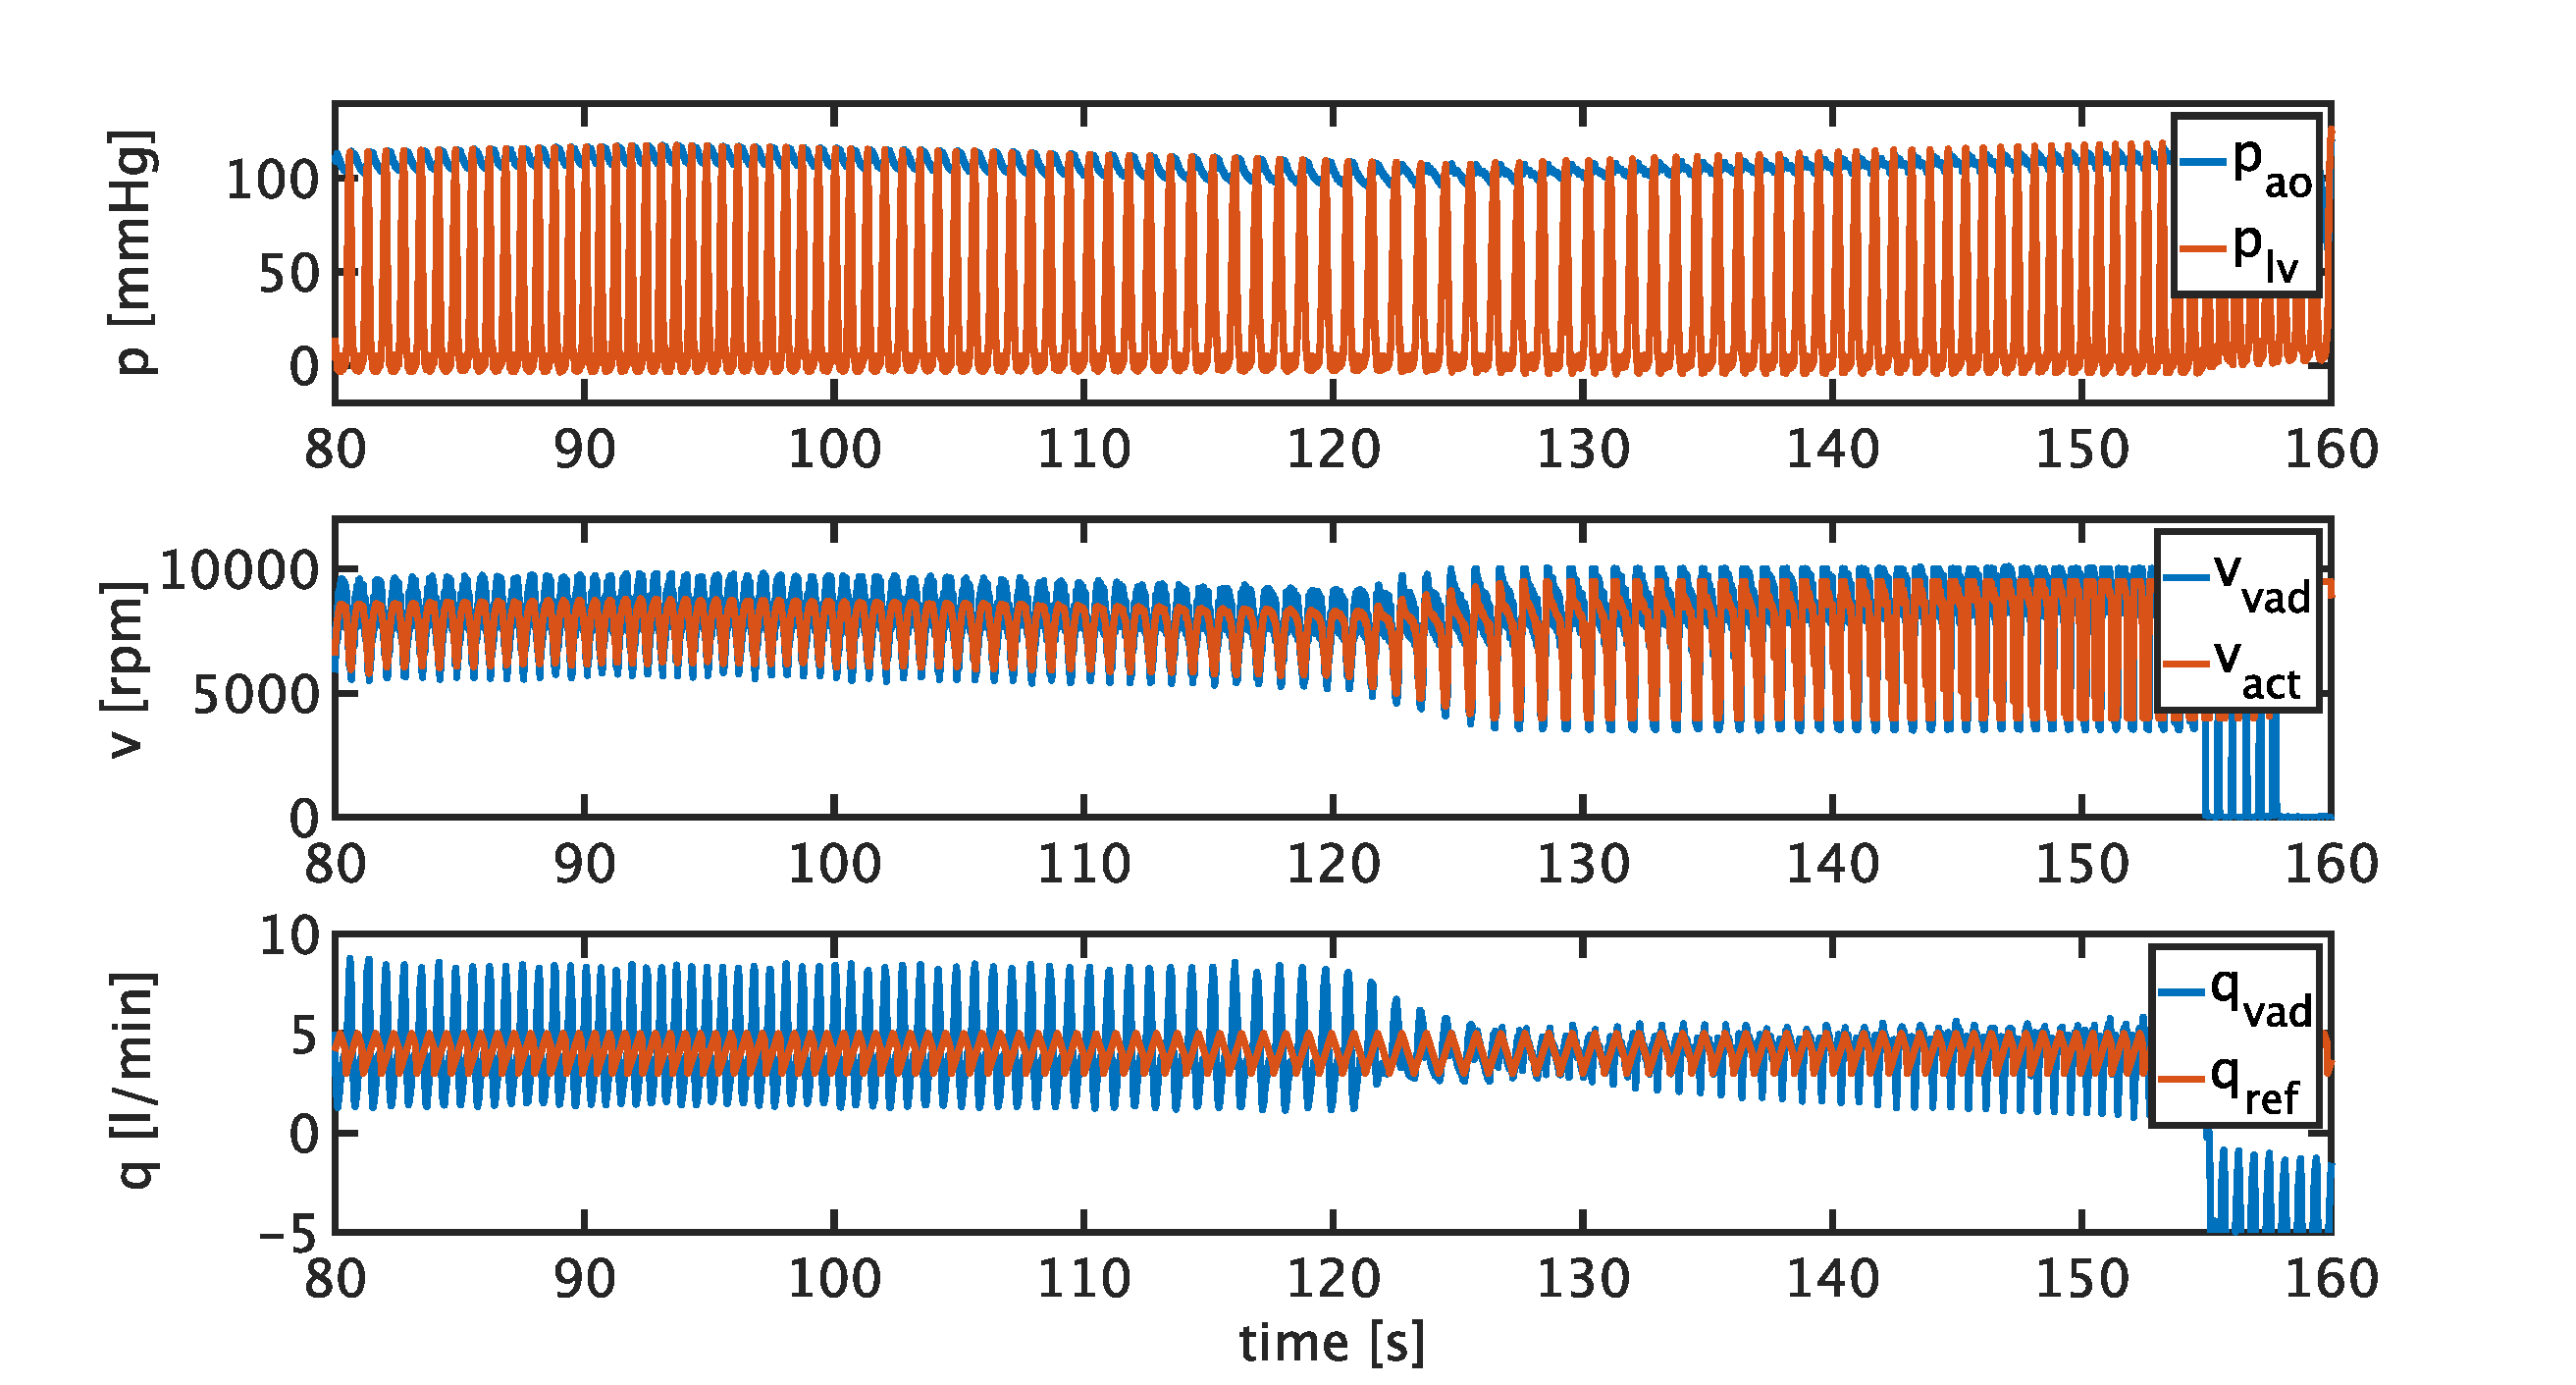
\includegraphics[width=0.95\textwidth]{images/chapt_5/ILC/ilc_var_dist_unfix_triang.pdf}
  \caption[Segment of measurement for ILC with varying disturbance with $cf_{\mathrm{Lv}}=1$ for triangular reference flow without data resampling]{Segment of measurement for ILC with varying disturbance with $cf_{\mathrm{Lv}}=1$ for triangular reference flow without data resampling. Top:  pressure values of the MCL. Middle: actuating variable and measured rotational speed of the VAD. Bottom: targeted flow trajectory and measured flow through the VAD}
  %\label{fig:ilc_var_dist_unfix_triang}
   \label{fig:anh_11}
\end{figure}

\begin{figure}[ht!]
  \centering
  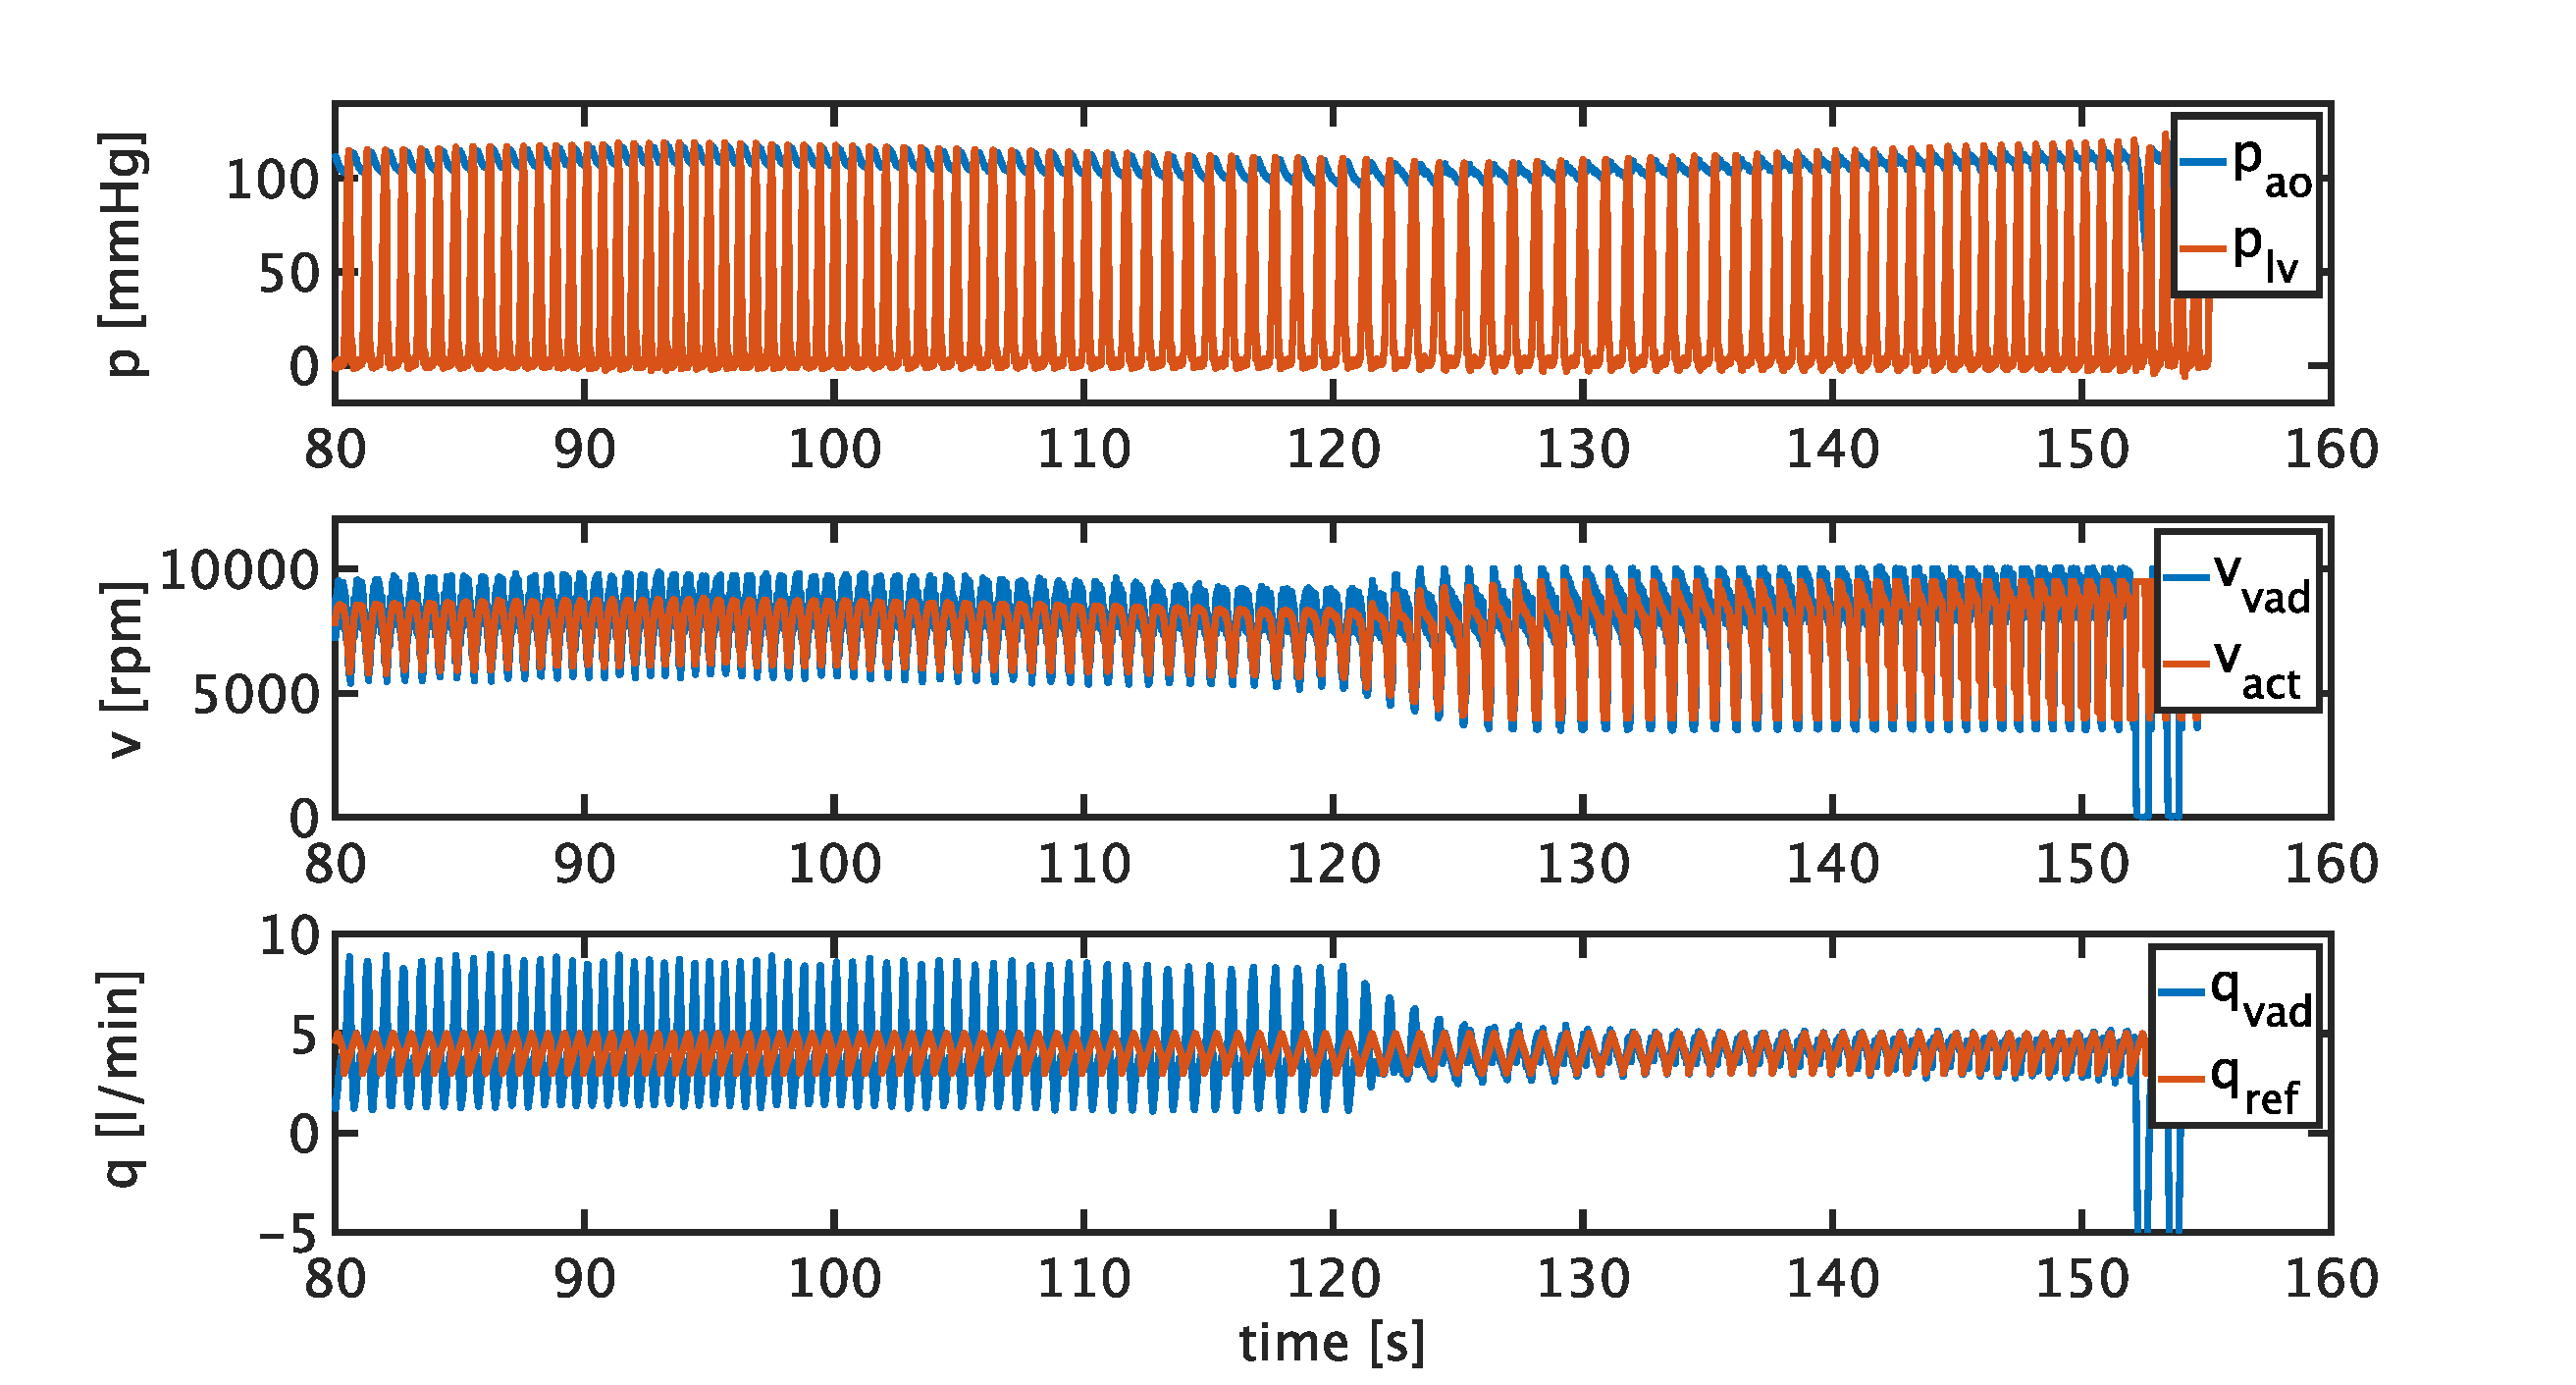
\includegraphics[width=0.95\textwidth]{images/chapt_5/ILC/ilc_var_dist_fix_triang.pdf}
  \caption[Segment of measurement for ILC with varying disturbance with $cf_{\mathrm{Lv}}=1$ for triangular reference flow with data resampling]{Segment of measurement for ILC with varying disturbance with $cf_{\mathrm{Lv}}=1$ for triangular reference flow with data resampling. Top:  pressure values of the MCL. Middle: actuating variable and measured rotational speed of the VAD. Bottom: targeted flow trajectory and measured flow through the VAD}
  %\label{fig:ilc_var_dist_fix_triang}
   \label{fig:anh_12}
\end{figure}

\begin{figure}[ht!]
  \centering
  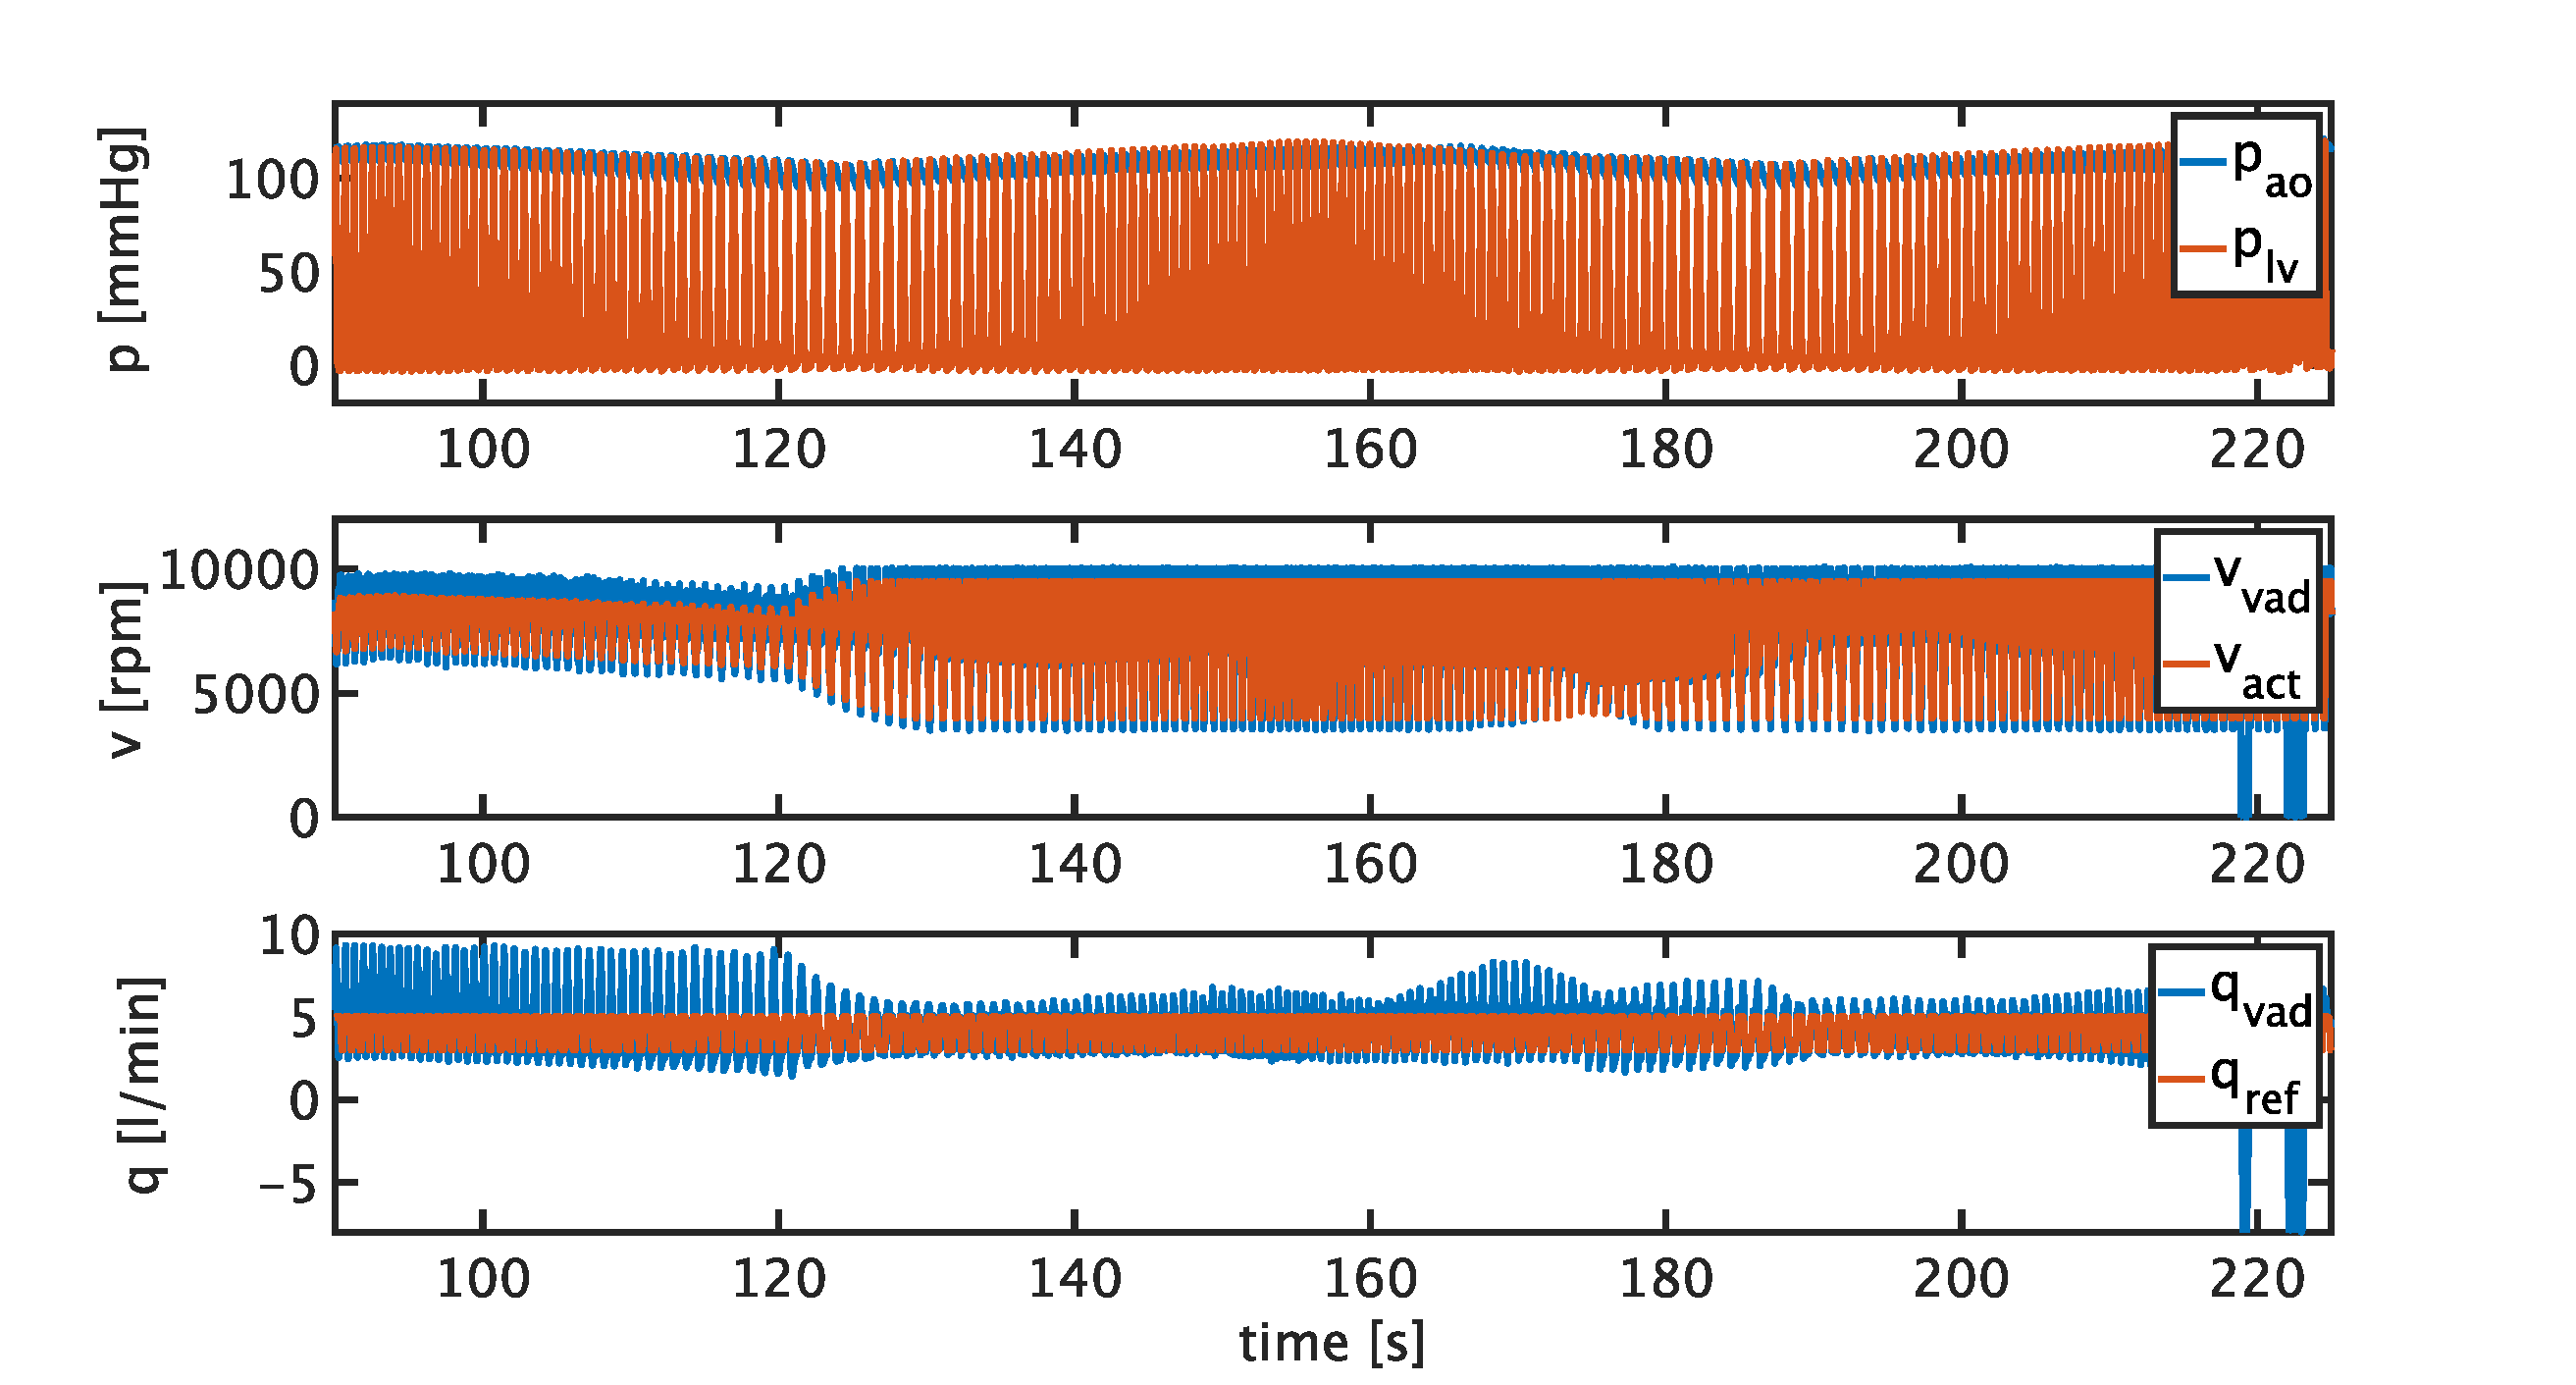
\includegraphics[width=0.95\textwidth]{images/chapt_5/ILC/ilc_var_dist_unfix_rect.pdf}
  \caption[Segment of measurement for ILC with varying disturbance with $cf_{\mathrm{Lv}}=1$ for rectangular reference flow without data resampling]{Segment of measurement for ILC with varying disturbance with $cf_{\mathrm{Lv}}=1$ for rectangular reference flow without data resampling. Top:  pressure values of the MCL. Middle: actuating variable and measured rotational speed of the VAD. Bottom: targeted flow trajectory and measured flow through the VAD}
  %\label{fig:ilc_var_dist_unfix_rect}
   \label{fig:anh_13}
\end{figure}

\begin{figure}[ht!]
  \centering
  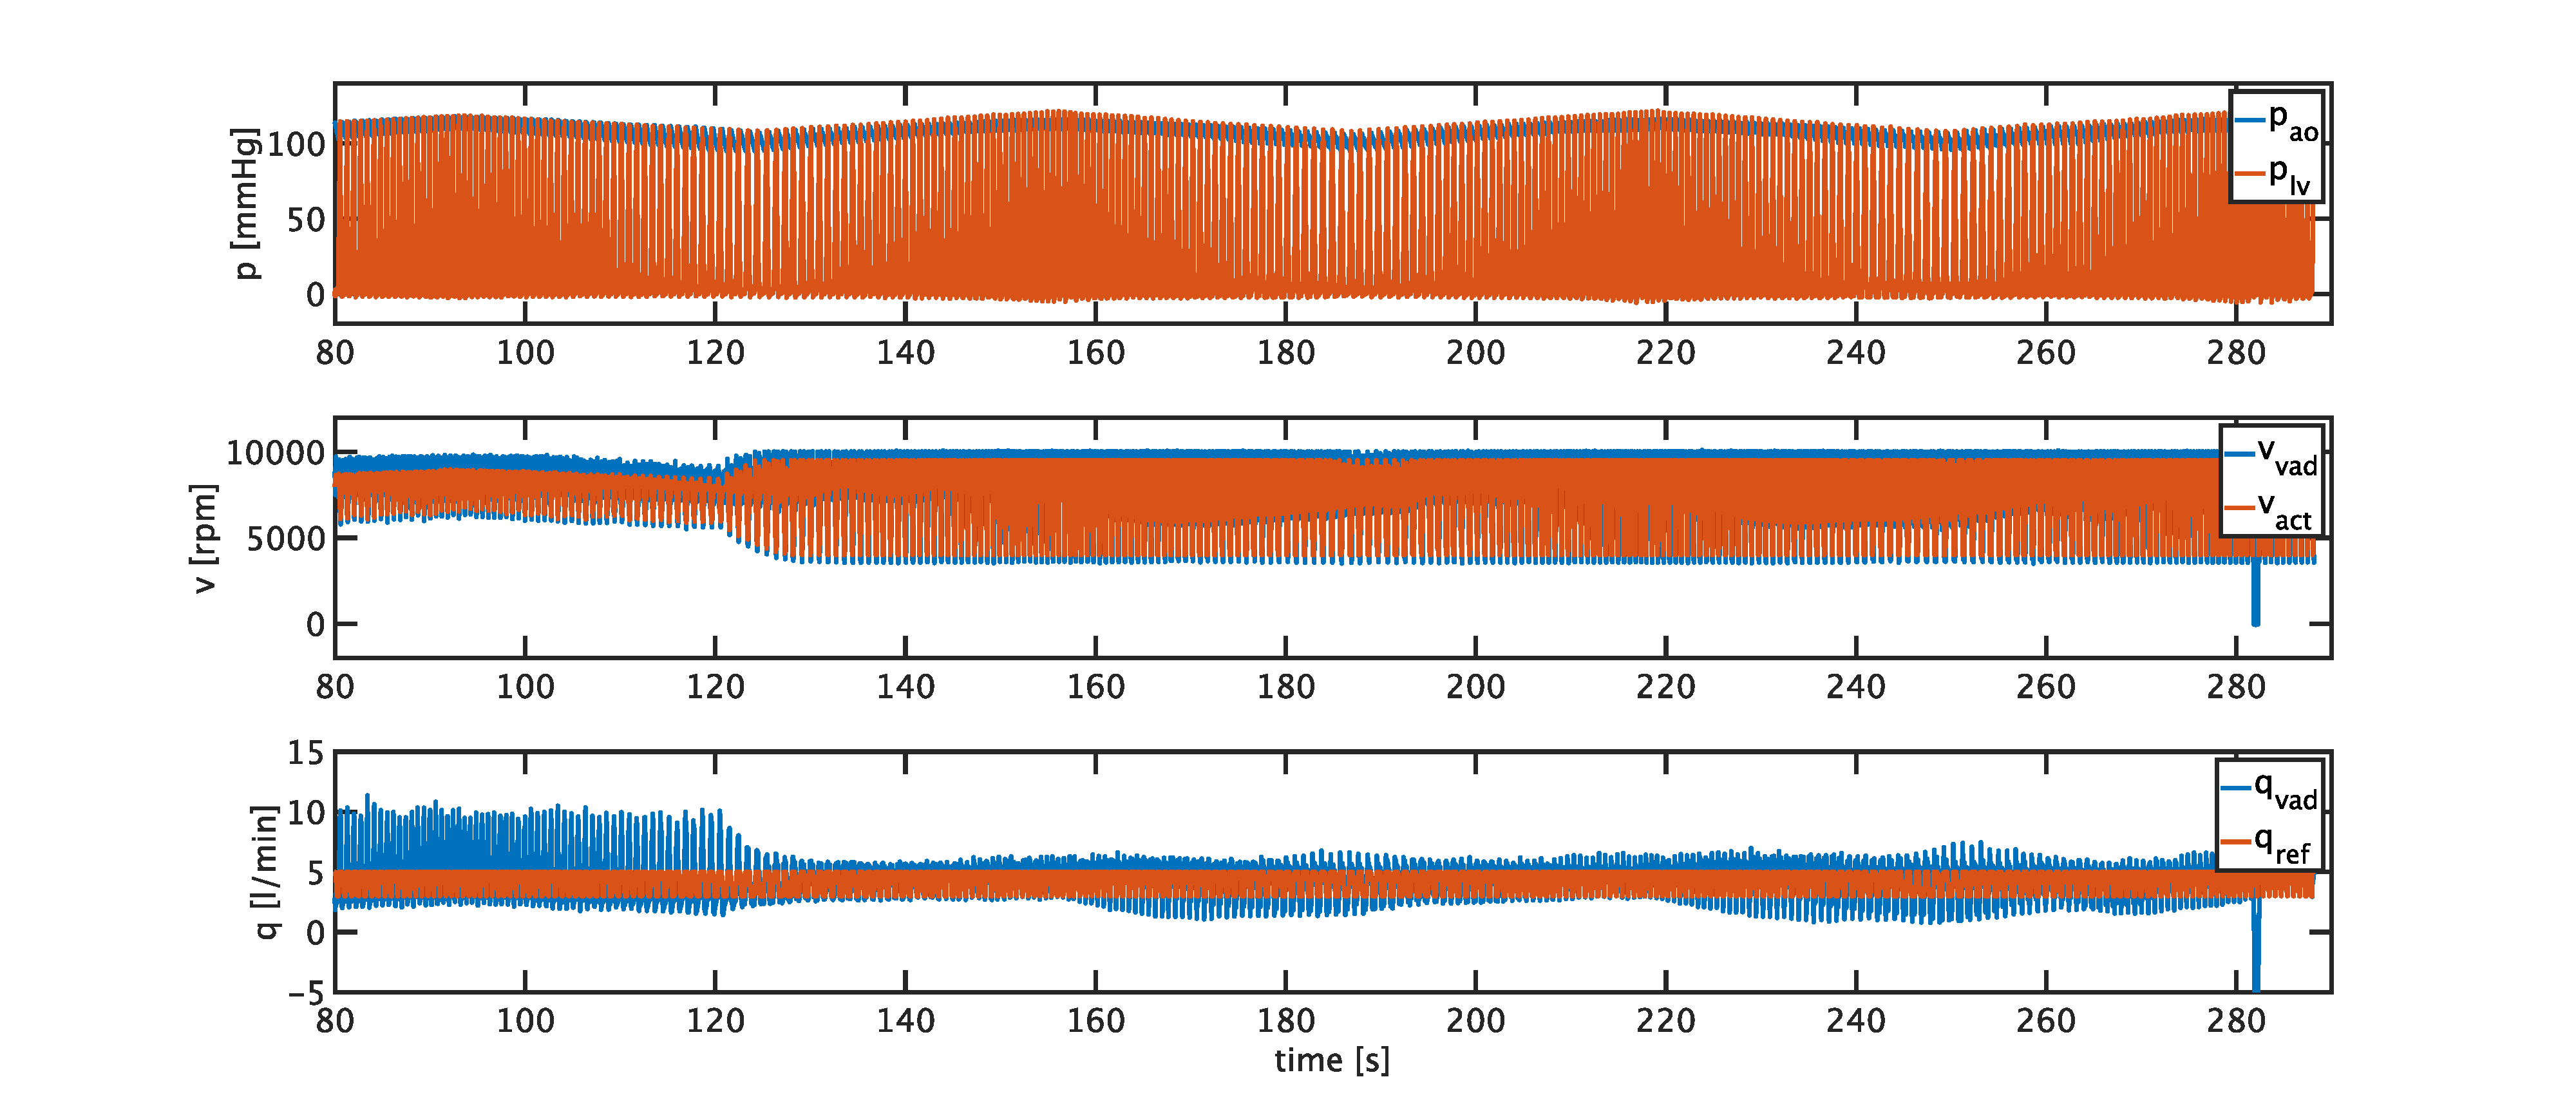
\includegraphics[width=0.95\textwidth]{images/chapt_5/ILC/ilc_var_dist_fix_rect.pdf}
  \caption[Segment of measurement for ILC with varying disturbance with $cf_{\mathrm{Lv}}=1$ for rectangular reference flow with data resampling]{Segment of measurement for ILC with varying disturbance with $cf_{\mathrm{Lv}}=1$ for rectangular reference flow with data resampling. Top:  pressure values of the MCL. Middle: actuating variable and measured rotational speed of the VAD. Bottom: targeted flow trajectory and measured flow through the VAD}
  %\label{fig:ilc_var_dist_fix_rect}
   \label{fig:anh_14}
\end{figure}
